%%%%%%%%%%%%%%%%%%%%%%%%%%%%%%%%%%%%%%%%%
% kaobook
% LaTeX Template
% Version 1.2 (4/1/2020)
%
% This template originates from:
% https://www.LaTeXTemplates.com
%
% For the latest template development version and to make contributions:
% https://github.com/fmarotta/kaobook
%
% Authors:
% Federico Marotta (federicomarotta@mail.com)
% Based on the doctoral thesis of Ken Arroyo Ohori (https://3d.bk.tudelft.nl/ken/en)
% and on the Tufte-LaTeX class.
% Modified for LaTeX Templates by Vel (vel@latextemplates.com)
%
% License:
% CC0 1.0 Universal (see included MANIFEST.md file)
%
%%%%%%%%%%%%%%%%%%%%%%%%%%%%%%%%%%%%%%%%%

%----------------------------------------------------------------------------------------
%	PACKAGES AND OTHER DOCUMENT CONFIGURATIONS
%----------------------------------------------------------------------------------------

\documentclass[
	fontsize=11pt, % Base font size
	twoside=true, % Use different layouts for even and odd pages (in particular, if twoside=true, the margin column will be always on the outside)
	%open=any, % If twoside=true, uncomment this to force new chapters to start on any page, not only on right (odd) pages
	%chapterprefix=true, % Uncomment to use the word "Chapter" before chapter numbers everywhere they appear
	%chapterentrydots=true, % Uncomment to output dots from the chapter name to the page number in the table of contents
	numbers=noenddot, % Comment to output dots after chapter numbers; the most common values for this option are: enddot, noenddot and auto (see the KOMAScript documentation for an in-depth explanation)
	%draft=true, % If uncommented, rulers will be added in the header and footer
	%overfullrule=true, % If uncommented, overly long lines will be marked by a black box; useful for correcting spacing problems
]{kaobook}

% Set the language
\usepackage[english]{babel} % Load characters and hyphenation
\usepackage[english=british]{csquotes} % English quotes

% Load packages for testing
\usepackage{blindtext}
%\usepackage{showframe} % Uncomment to show boxes around the text area, margin, header and footer
%\usepackage{showlabels} % Uncomment to output the content of \label commands to the document where they are used

% Load the bibliography package
\usepackage{styles/kaobiblio}
\addbibresource{main.bib} % Bibliography file

% Load mathematical packages for theorems and related environments. NOTE: choose only one between 'mdftheorems' and 'plaintheorems'.
\usepackage{styles/mdftheorems}
%\usepackage{styles/plaintheorems}

% Packages for sublists
\usepackage{enumitem}
\setlist[enumerate]{label*=\arabic*.}

\graphicspath{{examples/documentation/images/}{images/}} % Paths in which to look for images

\makeindex[columns=2, title=Alphabetical Index, intoc] % Make LaTeX produce the files required to compile the index

\makeglossaries % Make LaTeX produce the files required to compile the glossary

\makenomenclature % Make LaTeX produce the files required to compile the nomenclature

% Reset sidenote counter at chapters
%\counterwithin*{sidenote}{chapter}

%----------------------------------------------------------------------------------------

\begin{document}

%----------------------------------------------------------------------------------------
%	BOOK INFORMATION
%----------------------------------------------------------------------------------------

\titlehead{ShEx-Lite}
\subject{Final Degree Project}

\title[ShEx-Lite]{ShEx-Lite}
\subtitle{Automatic generation of domain object models through a subset of a Shape Expressions Compact Syntax.}

\author[Guillermo Facundo Colunga]{Guillermo Facundo Colunga}

\date{\today}

\publishers{School of Computer Science\\University of Oviedo}

%----------------------------------------------------------------------------------------

\frontmatter % Denotes the start of the pre-document content, uses roman numerals

%----------------------------------------------------------------------------------------
%	OPENING PAGE
%----------------------------------------------------------------------------------------

%\makeatletter
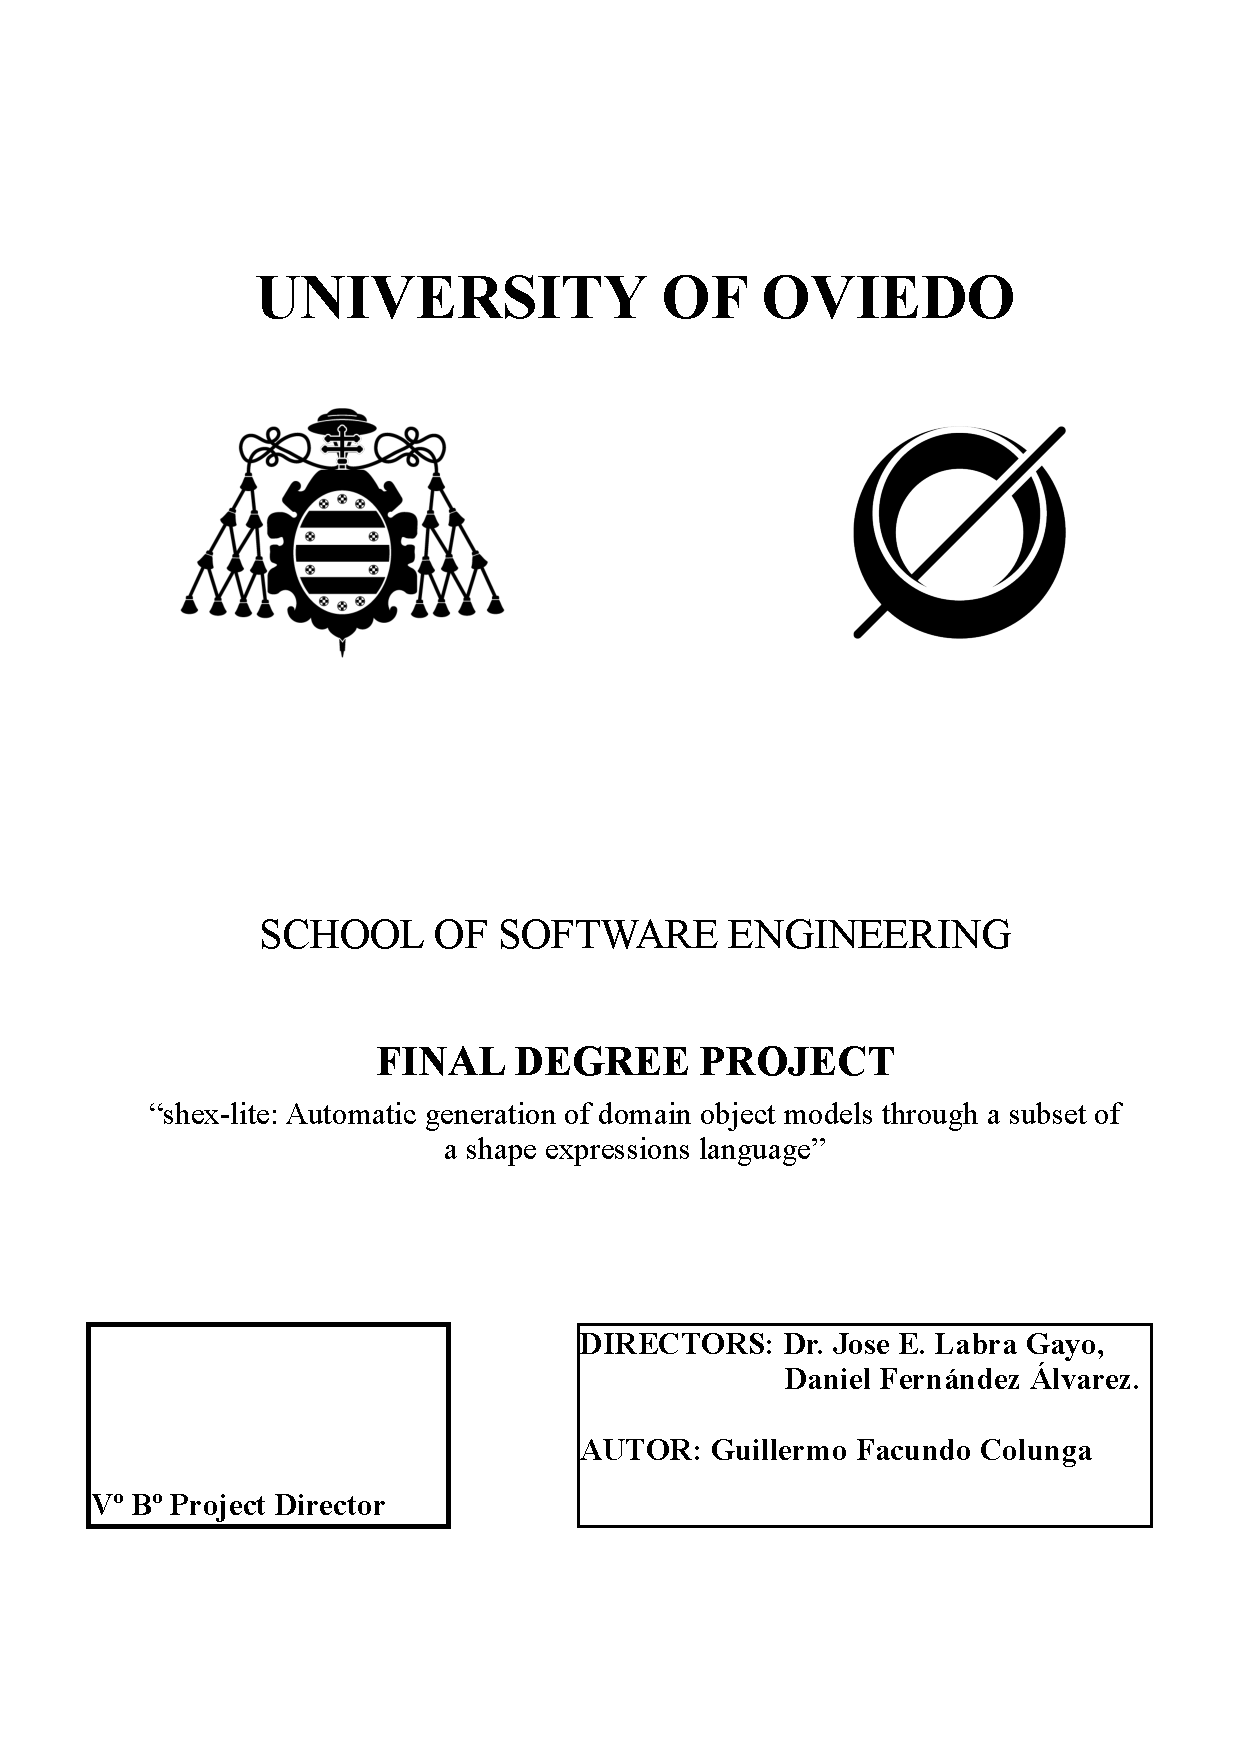
\includepdf{images/disertation-official-page.pdf}
%\makeatother

%----------------------------------------------------------------------------------------
%	COPYRIGHT PAGE
%----------------------------------------------------------------------------------------

\makeatletter
\uppertitleback{\@titlehead} % Header

\lowertitleback{
	Final Degree Project presented on July 2020 at the School of Software Engineering, Oviedo University. All the source code related to the implementation explored during this book is available at \url{github.com/weso/shex-lite}.

	\medskip

	\textbf{Copyright}\\
	All rights reserved. This project or any portion may not be reproduced or used in any manner without the express quotation to the original author.

	\medskip

	\textbf{Directors} \\
	Dr. Jose Emilio Labra Gayo\\Daniel Fernández Álvarez
}
\makeatother

%----------------------------------------------------------------------------------------
%	DEDICATION
%----------------------------------------------------------------------------------------

\dedication{
	The harmony of the world is made manifest in Form and Number, and the heart and soul and all the poetry of Natural Philosophy are embodied in the concept of mathematical beauty.\\
	\flushright -- D'Arcy Wentworth Thompson
}

%----------------------------------------------------------------------------------------
%	OUTPUT TITLE PAGE AND PREVIOUS
%----------------------------------------------------------------------------------------

% Note that \maketitle outputs the pages before here

% If twoside=false, \uppertitleback and \lowertitleback are not printed
% To overcome this issue, we set twoside=semi just before printing the title pages, and set it back to false just after the title pages
\KOMAoptions{twoside=semi} % default as 'semi' but turned to false so the first page is printed right after the cover, the cover is intended to be prented separetly.
\maketitle
\KOMAoptions{twoside=false}

%----------------------------------------------------------------------------------------
%	AKNOWLEDGEMENTS
%----------------------------------------------------------------------------------------

\chapter*{Aknowledgments}
\addcontentsline{toc}{chapter}{Aknowledgments} % Add the preface to the table of contents as a chapter

There are many people thanks to whom I write this work today. First of all I would like to thank my teachers Dr. Jose Emilio Labra Gayo and Daniel Fernández Álvarez, as well as the semantic web research group of the University of Oviedo for the trust placed in me to carry out this project.
However, this project is done as a summary of what has been my time at the university and a personal stage. That is why I would like to make a small dedication to those people who in one way or another have helped me to write this project today.
To my mother, Esther, for waiting until I was ready to leave us. To my uncle Andrés for being my guardian angel. To my grandparents, for giving me everything they had. To my coach Vic, who unwittingly has become a father to me. To Laura, the impossible girl. Ricardo, although I have never counted on you, you have always been. To Monica, for being you. To Pablo, without you I would not be who I am and I would never have finished this degree. To Álvaro, for letting me be your “manín". To Sari, for laughing at me when I needed it. To Cotito, for teaching me to accept myself. To Alejandro, for getting me out of my comfort zone. To Pablín, for being my prettiest doctor. To all my friends and family, those who I did not mention and those that I left along the way I dedicate this work to you for the moments you give me. And finally to my CAU family, thank you, really.
I hope that this work and I will not be a disappointment to any of you, really, each and every one of you are exceptional.

\begin{kaobox}[frametitle=Spanish]
	Son muchas las personas gracias a las que hoy escribo este trabajo. En primer lugar me gustaría agradecer a mis tutores Aquilino Juan Fuerte y Jose Emilio Labra Gayo, así como al grupo de investigación de web semántica de la Universidad de Oviedo y a Izertis S.A. la confianza depositada en mi para la realización de este proyecto.
	Sin embargo este proyecto se realiza como resumen de lo que ha sido mi paso por la universidad y por una etapa personal. Es por eso que me gustaría realizar una pequeña dedicatoria a aquellas personas que de una forma u otra han ayudado a que este escribiendo este proyecto hoy. A mi madre, Esther, por esperar a que estuviera preparado para marcharse. A mi tío Andrés por haber sido mi angel de la guarda. A mis abuelos, por dejarse la vida en mí. A mi entrenador Vic, quien sin quererlo se ha convertido en un padre. A Laura, la chica imposible. A Ricardo, aunque jamás he contado contigo siempre has estado. A Mónica, por ser tú. A Pablo, sin ti no sería quién soy y jamás habría terminado la carrera. A Álvaro, por dejarme ser tu manín. A Sari, por reñirme cuando lo necesitaba. A Cotito, por ser enseñarme a aceptarme. A Alejandro, por sacarme de mi zona de confort. A Pablín, por ser mi médico más cuqui. A todos mis amigos y amigas que dejé por el camino os dedico este trabajo por los momentos que me distéis. Y finalmente a mi familia del CAU, gracias, de verdad.
	Espero que este trabajo y yo no seamos una decepción para ninguno de vosotros, de verdad, todos y cada uno sois excepcionales.
\end{kaobox}

%----------------------------------------------------------------------------------------
%	ABSTRACT
%----------------------------------------------------------------------------------------

\chapter*{Abstract}
\addcontentsline{toc}{chapter}{Abstract} % Add the preface to the table of contents as a chapter

This end of degree project is about creating a compiler for a subset of the Shape Expressions Compact Syntax, focused on syntactic and semantic validation and the generation of domain models in object oriented languages. \todo{Completar...}


%----------------------------------------------------------------------------------------
%	TABLE OF CONTENTS & LIST OF FIGURES/TABLES
%----------------------------------------------------------------------------------------

\begingroup % Local scope for the following commands

% Define the style for the TOC, LOF, and LOT
%\setstretch{1} % Uncomment to modify line spacing in the ToC
%\hypersetup{linkcolor=blue} % Uncomment to set the colour of links in the ToC
\setlength{\textheight}{23cm} % Manually adjust the height of the ToC pages

% Turn on compatibility mode for the etoc package
\etocstandarddisplaystyle % "toc display" as if etoc was not loaded
\etocstandardlines % toc lines as if etoc was not loaded

\tableofcontents % Output the table of contents

\listoffigures % Output the list of figures

% Comment both of the following lines to have the LOF and the LOT on different pages
\let\cleardoublepage\bigskip
\let\clearpage\bigskip

\listoftables % Output the list of tables

\endgroup

%----------------------------------------------------------------------------------------
%	MAIN BODY
%----------------------------------------------------------------------------------------

\mainmatter % Denotes the start of the main document content, resets page numbering and uses arabic numbers
\setchapterstyle{kao} % Choose the default chapter heading style

\setchapterpreamble[u]{\margintoc}
\chapter{Introduction}
\labch{intro}

\textit{This project was born in the bar of a pub where the parents of RDF graph validation were talking about creating a tool that would allow people who were not computer-scientist to get started and later work with RDF graph validation schemes.}

% The motivation section.
\section{Motivation}\labsec{ch01-motivation}

Each day more and more devices generate data both automatically and manually, and also each day the development of application in different domains that are backed by databases and expose these data to the web becomes easier. The amount and diversity of data produced clearly exceeds our capacity to consume it.

To describe the data that is so large and complex that traditional data processing applications can’t handle the term big data \sidecite[-100pt]{big-data} has emerged. Big data has been described by at least three words starting by V: volume, velocity, variety. Although volume and velocity are the most visible features, variety is a key concept which prevents data integration and generates lots of interoperability problems.

In order to solve this key concept RDF (Resource Description Framework) was proposed as a graph-based data model \sidecite[-150pt]{graph-data-model} which became part of the Semantic Web \sidecite[-125pt]{semantic-web} vision. Its reliance on the global nature of URIs\sidenote[][-100pt]{A Uniform Resource Identifier (URI) is a string of characters that unambiguously identifies a particular resource. To guarantee uniformity, all URIs follow a predefined set of syntax rules, but also maintain extensibility through a separately defined hierarchical naming scheme.\\Ref.\url{https://en.wikipedia.org/wiki/Uniform_Resource_Identifier}} offered a solution to the data integration problem as RDF datasets produced by different means can seamlessly be integrated with other data.

Also, and related to his is the concept of Linked Data \sidecite{linked-data} that was proposed as a set of best practices to publish data on the Web. It was introduced by Tim Berners-Lee and was based on four main principles:

\begin{itemize}
  \item Use URIs as names for things.
  \item Use HTTP URIs so that people can look up those names.
  \item When someone looks up a URI, provide useful information, using the standards (RDF, SPARQL).
  \item Include links to other URIs. so that they can discover more things.
\end{itemize}

\begin{marginfigure}
	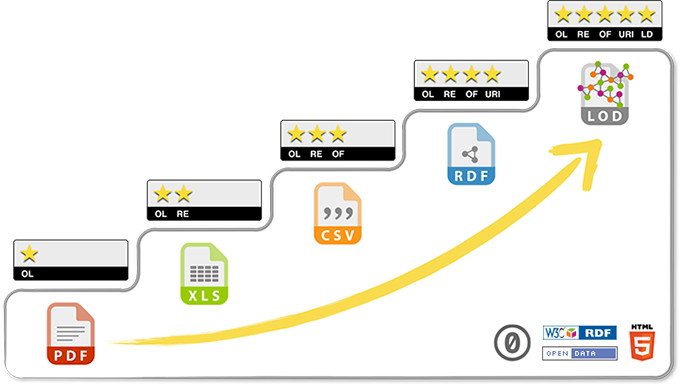
\includegraphics{5-star-steps}
	\caption[The 5 star steps of Linked Data]{The 5 star steps of Linked Data.}
	\labfig{margin-5-star-steps}
\end{marginfigure}

This four principles are called the 5 stars Linked Open Data Model, illustrated in \reffig{margin-5-star-steps}.
RDF is mentioned in the third principle as one of the standards that provides useful information. The goal of this principles is that data is not only ready for humans to navigate through but also for other agents, like computers, that may automatically process that data.

All the above motivations helped to make RDF the language for the Web of Data, as described in \sidecite{labra-validating-rdf}. And the main features that it presents are: Disambiguation, Integration, Extensibility, Flexibility and Open by Default. All this concepts will be deeply explored in \refsec{ch02-rdf}, but with the features also some drawbacks are associated, the most important one and the one we will focus is the RDF production/consumption dilema.

RDF production/consumption dilema states that it is necessary to find ways that data producers can generate their data so it can be handled by potential consumers. For example, they may want to declare that some nodes have some properties with some specific values. Data consumers need to know that structure to develop applications to consume the data.

Although RDF is a very flexible schema-less language, enterprise and industrial applications may require an extra level of validation before processing for several reasons like security, performance, etc.

To solve that dilema and as an alternative to expecting the data to have some structure without validation, Shape Expressions (ShEx) where proposed as a human-readable and high-level open source language for RDF validation. Initially ShEx was proposed as a human-readable syntax for OSLC Resource Shapes \sidecite{oslc-resource-shape} but ShEx grew very fast to embrace more complex user requirements coming from clinical and library use cases.

Another technology, SPIN, was used for RDF validation, principally in TopQuadrant’s TopBraid Composer. This technology, influenced from OSLC Resource Shapes as well, evolved into both a private implementation and open source definition of the Shapes Constraint Language (SHACL), which was adopted by the W3C Data Shapes Working Group.

From a user point of view the possibilities of ShEx are very large, from the smallest case to just validate a node with one property to a scientific domain case where we need to validate the human genome (a real use case of ShEx). As seen, ShEx is a new powerful language, but it can became complicated on the corner cases, but most of day-to-day uses can be solved with a subset of the language. This is the point where this project borns. We will call this subset ShEx-Lite. The simplicity of ShEx-Lite is not only focus on computer scientists who have experience the pain of new languages but also for other non-technical profiles that need to validate RDF data.

Besides to this, a common problem is that some companies use ShEx to define the constraints of the RDF data that they own. But then, when developing applications with object oriented languages they need to translate those schemas in to a domain model to support their data. Furthermore if the Shape Expressions used to validate their data changes for some reason they need to rewrite that domain model in the OOL again.

Finally, from a ShEx developer point of view sometimes appears the need to try new features in a small playground that allow easy an fast testing.


% The purpose section.
\section{Main usage scenarios}\labsec{ch01-main-usage-scenarios}

\refsec{ch01-motivation} introduced some profiles that might benefit from using ShEx-Lite. We can find an example of this profiles in the Wikidata Community. Wikidata is formed by a multidisciplinar community whose aim is to introduce RDF data in to an open knowledge base used by other companies like Google Search. The only problem is that the introduced RDF data needs validation to ensure a minimum data quality, but the profiles that introduce the data, usually, are domain experts whose knowledge about computer science is limited. \todo{Extender ejemplo wikidata.}

Besides to this, a common problem is that some companies like Wikidata or even Universities use ShEx to define the constraints of the RDF data that they own. But then, when developing applications with object oriented languages they need to translate those schemas in to a domain model to support their data. Furthermore if the Shape Expressions used to validate their data changes for some reason they need to rewrite that domain model in the OOL again. \todo{Adornar un poco.}

Finally, from a ShEx developer point of view sometimes appears the need to try new features in a small playground that allow easy an fast testing, for example a feature that appeared after this project was implemented is to automatically generate documentation webpages for the schemas defined in ShEx, but the first target of this feature won’t be ShEx, will be ShEx-Lite as it is perfect for he proof of concept.

\todo{Enumerar tipos de erramientas que se beneficiarían.}


% The contents of the proposal section.
\section{Content of the proposal}\labsec{ch01-content-of-the-proposal}

After \refsec{ch01-motivation} and \refsec{ch01-main-usage-scenarios} this section descibes the developed system to solve the deficiencies and different profile-users requests.

\begin{description}
  \item[First] A compiler for a language defined as a subset of the shape expressions language focused on helping the non-expert user on solving problems with their schemas.
  \item[Secondly] A functionality in this compiler, that allows to automatically create domain object models in object-oriented programming languages, from the defined schemas.
\end{description}

\subsection{ShEx-Lite Compiler}
This compiler works over a defined subset of the Shape Expressions Compact Syntax, defined at \sidecite{shexc} that allows expressing basic constraints. It is implemented with the paradigm "compiler as a library" because the influence of modern compilers like Swift, Rust or Roslyn \sidecite{swift, rustc,dotNet} and it is able to parse a schema, analyze it and generate the syntactic and semantic errors that the schema contains.

The ShEx-Lite Compiler is composed of the following components:

\subsubsection{Syntax analysis}
The syntax analysis phase covers the transformation of the input in to an Abstract Syntax Tree. That is, lex and parse the file, generate the parse tree, raise any errors or warnings and finally build the AST.

\subsubsection{Semantic analysis}
The semantic analysis covers the validation and transformation of the AST in to the SIL (ShEx-Lite Intermediate Language). Is during this stage where the AST gets validated, type-checked and transformed from a tree to a graph, is this graph the one that gets the name of SIL.




\subsection{Automatic generation of domain object models}
But by far, the biggest difference with existing tools, is the automatic generation of domain object models from the schemas defined.

The idea behind this is to enhance interoperability between object oriented languages \sidecite[-15pt]{oopl} and RDF systems. An example of this is the European Project ASIO Hércules \sidecite{hercules-um}, where the automatic transformation of schemas in to POJOs \sidecite{pojo} is the tool that joins the Semantic Architecture and the Ontology Infrastructure.

Also it is important to remark here that we are perfectly conscious about the fact that not every object oriented language allows to model exactly the same restrictions as types differ, therefore each OOL needs to validate or map the schema to a representation on the language whose meaning is the same, that is create the image of the schema in the corresponding language.


% The contents section.
\section{Structure}\labsec{ch01-structure}
The project layout is as follows:\\

\begin{description}
	\item[Chapter 2] Indicates the state of the art of the existing RDF validation technologies, tools for processing Shape Expressions and other related projects.
	\item[Chapter 3] Describes the goals that the project aim to achieve after its execution and possible real-world applications.
	\item[Chapter 4] Contains a detailed initial planning and budget for the project, this is the designed planning followed during the execution of the project and the initial estimated budget.
	\item[Chapter 5] Gives a basic theoretical background that it is needed to fully understand the concepts explained in the following chapters.
	\item[Chapter 6] Provides a technical description of the design and implementation of the compiler itself. This includes, analysis, design, the technological stack choices, diagrams, implementation decisions and tests.
	\item[Chapter 7] Compares the initial planning developed in chapter 4 with the final one. This includes the genuine execution planning of the project and the reasons and events that modified the one from chapter 4.
	\item[Chapter 8] Summarizes the analysis and results given over the project, gives an outlook for future work continuing the development of the implemented solution. And includes the diffusion of results done during the project.
	\item[Chapter 9] Includes all the set of references used during this document. It is fully recommended to read them carefully and use them as source of truth for any doubt.
	\item[Chapter 10] Attaches every document related to the project and referenced from other chapters that has been developed during the project. Here we include detailed budget, system manuals, and other documents.
\end{description}


\setchapterpreamble[u]{\margintoc}
\chapter{Theoretical Background}
\labch{theory}

For a proper understanding of this documentation and the ideas explained on it it is needed to know some theoretical concepts that are the fundaments of Linked Data, RDF, RDF Validation, programing languages and compilers. This sections is devoted to carefully explain those concepts to the needed deepth to fully understand this dissertation, but for those readers that want a deeper explanation a more detailed view of the concepts presented here is offered in \sidecite{labra-validating-rdf, eric-rdf-validation-lang, programing-language}.

% Section 1, RDF.
\section{RDF}
\labsec{ch02-rdf}
Resource Description Framework (RDF) is a standard model for data interchange on the web, started in 1998 and the first version of the specification was published in 2004 by the W3C according to \sidecite{rdf-primer}. RDF has features that facilitate data merging even if the underlying schemas differ, and it specifically supports the evolution of schemas over time without requiring all the data consumers to be changed. Another important feature is that RDF supports XML, N-Triples and Turtle syntax, the \reffig{rdf-ntriples-ex} shows an example of how a triplet can be written in RDF N-Triples Syntax.

\begin{figure}[hb]
\begin{lstlisting}
<http://example/subject1> <http://example/predicate1> <http://example/object1>
\end{lstlisting}
\caption[RDF N-Triples Example]{RDF N-Triples Example. From this example we can see that each triplet is composed of three elements, the subject the predicate and the object.}
\labfig{rdf-ntriples-ex}
\end{figure}

RDF extends the linking structure of the Web to use URIs to name the relationship between things as well as the two ends of the link (this is usually referred to as a “triple” or "triplet"). Using this simple model, it allows structured and semi-structured data to be mixed, exposed, and shared across different applications. \reffig{rdf-graph} shows an example of how different triples can be use to compose a graph, this graph represents the same as the \reffig{rdf-ntriples-graph}

\begin{figure}[hb]
\begin{lstlisting}
<http://example/bob> <http://example/knows> <http://example/alice> .
<http://example/alice> <http://example/knows> <http://example/peter> .
\end{lstlisting}
\caption[RDF N-Triples Graph Example]{RDF N-Triples Graph Example. This exmaple shows the n-triples that generate the graph from \reffig{rdf-graph}.}
\labfig{rdf-ntriples-graph}
\end{figure}

This linking structure forms a directed, labeled graph, where the edges represent the named link between two resources, represented by the graph nodes. This graph view is the easiest possible mental model for RDF and is often used in easy-to-understand visual explanations.

Also, related to this we strongly recommend the Tim Berners-Lee’s writings on Web Design Issues \sidecite{semantic-roadmap} where he explain the issues of the liked data and why is RDF so important.

\begin{marginfigure}
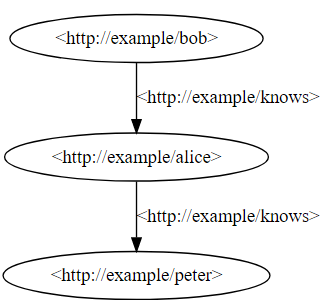
\includegraphics{rdf-graph}
\caption[RDF Example graph]{RDF Example graph.}
\labfig{rdf-graph}
\end{marginfigure}


% Section 2, Validating RDF.
\section{Validating RDF}
RDF therefore allows to represent and store data, and with this ability emerges the need to validate that the schema of the graph is correct. In order to perform the validation of RDF data there  have been previous attempts, described in \refsec{ch02-validating-other-techs}, this dissertation will focus on Shape Expressions. But in order to validate RDF data every technology will need to face the following RDF concepts:

\begin{itemize}
 \item the form of a node (the mechanisms for doing this will be called “node constraints”);
 \item the number of possible arcs incoming/outgoing from a node; and
 \item the possible values associated with those arcs.
\end{itemize}

\begin{figure}[hb]
  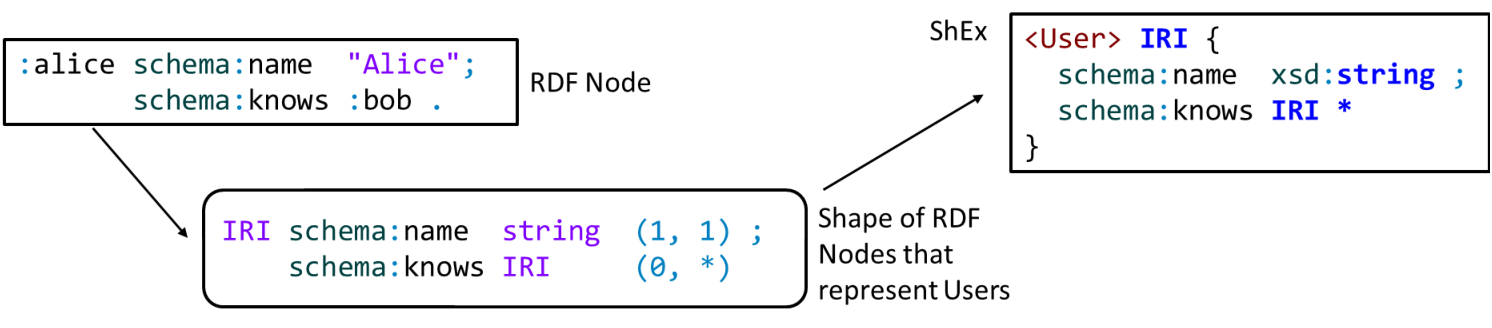
\includegraphics{rdf-node-and-shape}
  \caption[RDF node and its shape]{RDF node and its shape.}
  \labfig{rdf-graph}
\end{figure}

\reffig{rdf-graph} illustrates those RDF concepts by means of the Shape Expression that validates users. There we can see that the shape of the RDF node that represents Users represents the form of a node, the number of possible arcs and the possible value associated with those arcs.

\subsection{Shape Expressions}
As defined in \sidecite{labra-validating-rdf} Shape Expressions (ShEx) is a schema language for describing RDF graphs structures. ShEx was originally developed in late 2013 to provide a human-readable syntax for OSLC Resource Shapes. It added disjunctions, so it was more expressive than Resource Shapes. Tokens in the language were adopted from Turtle and SPARQL with tokens for grouping, repetition and wildcards from regular expression and RelaxNG Compact Syntax \sidecite{van2003relax}. The language was described in a paper \sidecite{eric-rdf-validation-lang} and codified in a June 2014 W3C member submission which included a primer and a semantics specification. This was later deemed “ShEx 1.0”.

As of publication, the ShEx Community Group was starting work on ShEx 2.1 to add features like value comparison and unique keys. See the ShEx Homepage \url{http://shex.io/} for the state of the art in ShEx. A collection of ShEx schemas has also been started at \url{https://github.com/shexSpec/schemas}.

\begin{figure}[hb]
\begin{lstlisting}
PREFIX :       <http://example.org/>
PREFIX schema: <http://schema.org/>
PREFIX xsd:  <http://www.w3.org/2001/XMLSchema#>

:User {
  schema:name          xsd:string  ;
  schema:birthDate     xsd:date?  ;
  schema:gender        [ schema:Male schema:Female ] OR xsd:string ;
  schema:knows         IRI @:User*
}
\end{lstlisting}
\caption[Shape Expression Example]{Shape Expression Example. This example describes a shape expression that describes a user as a node that has one name of type string, an optional bithd date of type date, one gender of type Male, Female or free string and a set between 0 and infinite of other users represented by the knows property.}
\labfig{shape-expr-ex}
\end{figure}

\subsubsection{ShEx Compact Syntax: \texttt{ShExC}}
The ShEx compact syntax (ShExC) was designed to be read and edited by humans. It follows some conventions which are similar to Turtle or SPARQL.

\begin{itemize}
	\item \texttt{PREFIX} and \texttt{BASE} declarations follow the same convention as in Turtle. In the rest of this chapter we will omit prefix declarations for brevity.
	\item Comments start with a \texttt{\#} and continue until the end of line.
	\item The keyword a identifies the \texttt{rdf:type} property.
	\item Relative and absolute IRIs are enclosed by \texttt{< >} and prefixed names (a shorter way to write out IRIs) are written with prefix followed by a colon.
	\item Blank nodes are identified using \texttt{\_:label} notation.
	\item Literals can be enclosed by the same quotation conventions ( \texttt{'}, \texttt{"}, \texttt{'''}, \texttt{"""}) as in Turtle.
	\item Keywords (apart from a) are not case sensitive. Which means that \texttt{MinInclusive} is the same as \texttt{MININCLUSIVE}.
\end{itemize}

A ShExC document declares a ShEx schema. A ShEx schema is a set of labeled shape expressions which are composed of node constraints and shapes. These constrain the permissible values or graph structure around a node in an RDF graph. When we are considering a specific node, we call that node the focus node.

\begin{figure}[hb]
  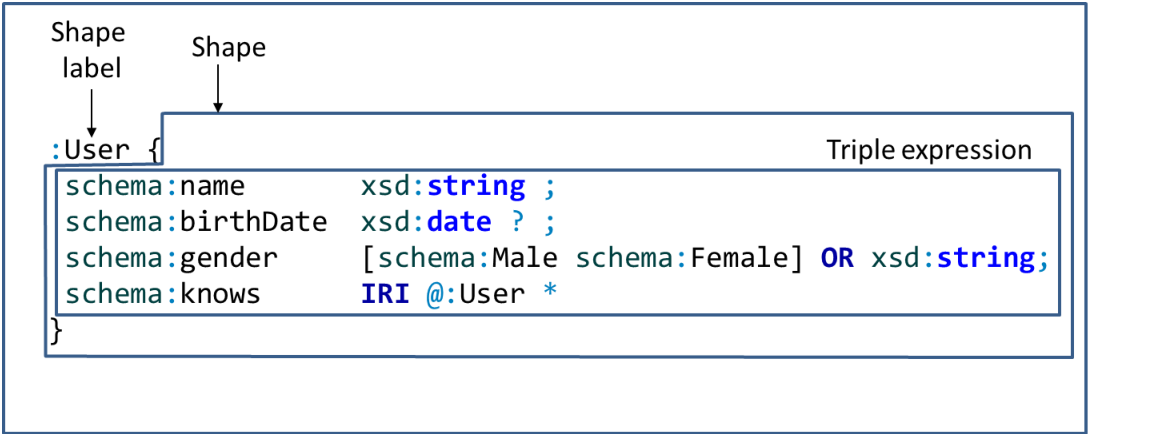
\includegraphics{shex-out}
  \caption[Shapes, shape expression labels and triple expressions]{Shapes, shape expression labels and triple expressions.}
  \labfig{shex-out-view}
\end{figure}

\reffig{shex-out-view} shows the first level of a shape expression, we have a label and the shape itself that is what we asing to the \texttt{:User} label. Then, the shape is composed by triple expressions. The triple expression structure is explained in \reffig{shex-triple-expression}, and as its name indicates it is composed of three elements, the property, the node constraint and the cardinality.

\begin{figure}[hb]
  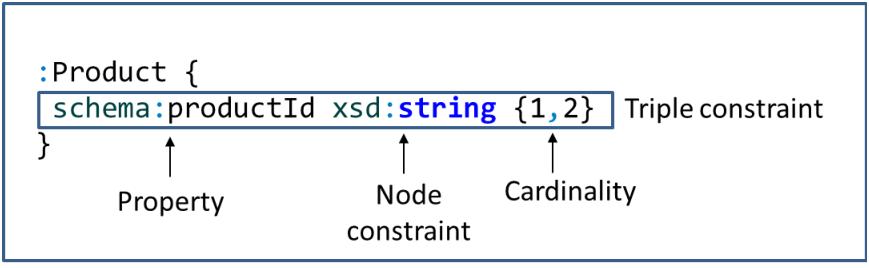
\includegraphics{shex-triple-expression}
  \caption[Parts of a triple expression]{Parts of a triple expression.}
  \labfig{shex-triple-expression}
\end{figure}

Shape Expressions Compact Syntax is much bigger and containts other multiple features that give ShEx its power, and all of them can be explored in \sidecite{labra-validating-rdf} but they are not needed to understand this dissertation.

\subsubsection{Use of ShEx}
Strictly speaking, a ShEx schema defines a set of graphs. This can be used for many purposes, including communicating data structures associated with some process or interface, generating or validating data, or driving user interface generation and navigation. At the core of all of these use cases is the notion of conformance with schema. Even one is using ShEx to create forms, the goal is to accept and present data which is valid with respect to a schema.
ShEx has several serialization formats:

\begin{itemize}
	\item a concise, human-readable compact syntax (ShExC);
	\item a JSON-LD syntax (ShExJ) which serves as an abstract syntax; and
	\item an RDF representation (ShExR) derived from the JSON-LD syntax.
\end{itemize}

These are all isomorphic and most implementations can map from one to another.
Tools that derive schemas by inspection or translate them from other schema languages typically generate ShExJ. Interactions with users, e.g., in specifications are almost always in the compact syntax ShExC. As a practical example, in HL7 FHIR, ShExJ schemas are automatically generated from other formats, and presented to the end user using compact syntax. See Section 6.2.3 for more details.
ShExR allows to use RDF tools to manage schemas, e.g., doing a SPARQL query to find out whether an organization is using dc:creator with a string, a foaf:Person, or even whether an organization is consistent about it.

\subsubsection{ShEx Implementations} \todo{Check links.}
At the time of this writing, we are aware of the following implementations of ShEx.

\begin{itemize}
	\item shex.js for Javascript/N3.js (Eric Prud’hommeaux) \url{https://github.com/shexSpec/shex.js/};
	\item Shaclex for Scala/Jena (Jose Emilio Labra Gayo) \url{https://github.com/labra/shaclex/};
	\item shex.rb for Ruby/RDF.rb (Gregg Kellogg) \url{https://github.com/ruby-rdf/shex};
	\item Java ShEx for Java/Jena (Iovka Boneva/University of Lille) \url{https://gforge.inria.fr/projects/shex-impl/}; and
	\item ShExkell for Haskell (Sergio Iván Franco and Weso Research Group) \url{https://github.com/weso/shexkell}.
\end{itemize}

There are also several online demos and tools that can be used to experiment with ShEx.

\begin{itemize}
	\item shex.js (http://rawgit.com/shexSpec/shex.js/master/doc/shex-simple.html);
	\item Shaclex (http://shaclex.herokuapp.com); and
	\item ShExValidata (for ShEx 1.0) (https://www.w3.org/2015/03/ShExValidata/).
\end{itemize}

\subsection{Other Technologies}\labsec{ch02-validating-other-techs}
As other validation technologies we will just explore the existence of them as it is very interesting to know how other tools approach the same issue.

\subsubsection{SHACL}
Also in \sidecite{labra-validating-rdf}, Chapter 5, it is fully explained that Shapes Constraint Language (SHACL) has been developed by the W3C RDF Data Shapes Working Group, which was chartered in 2014 with the goal to “produce a language for defining structural constraints on RDF graphs \sidecite{oslc-resource-shape}.”
The main difference that made us choose ShEx over SHACL are that ShEx emphasized human readability, with a compact grammar that follows traditional language design principles and a compact syntax evolved from Turtle.

\subsubsection{JSON Schema}
JSON Schema born as a way to validate JSON-LD, and as turtle and RDF can be serialized as JSON-LD it is usual to think that JSON Schema can validate RDF data, but this is not fully correct. And the reason is that the serialization of RDF data in to JSON-LD is not deterministic, that means that a single schema might have multiple serializations, which interferes with the validation as you cannot define a relative schema.


% Section 3, Programming Languages.
\section{Programming Languages}
According to [20] “a programming language is a formal language comprising a set of instructions that produce various kinds of output.” When we talk about programming languages we need to know that they are split into two, General Purpose Languages (GPL) and Domain Specific Languages (DSL). The main difference overtime is that, as said in [21], a domain-specific language (DSL) is a computer language specialized to a particular application domain in contrast to a general-purpose language (GPL), which is broadly applicable across domains.
In the specific case of ShEx-Lite we will be talking about a Domain Specific Language, and more deep we would classified it as a Declarative one, that means that it is not Touring Complete [22].


% Section 4, Compilers.
\section{Compilers}
A compiler is a computer program that translates computer code written in one programming language (the source language) into another language (the target language). Is during this translation process where the compiler validates the syntax and the semantics of the program, if any error is detected in the process the compiler raises an exception (understand as a compiler event that avoids the compiler to continue its execution).

\subsection{Internal Structure}
In order to decompose the internal structure of a compiler they have been split in to the most common task they do \reffig{compiler-stages}, of course this doesn’t mean that there are compilers with more or less stages, but at the end everything can be group into any of the groups that we will explain:

\begin{figure}[hb]
  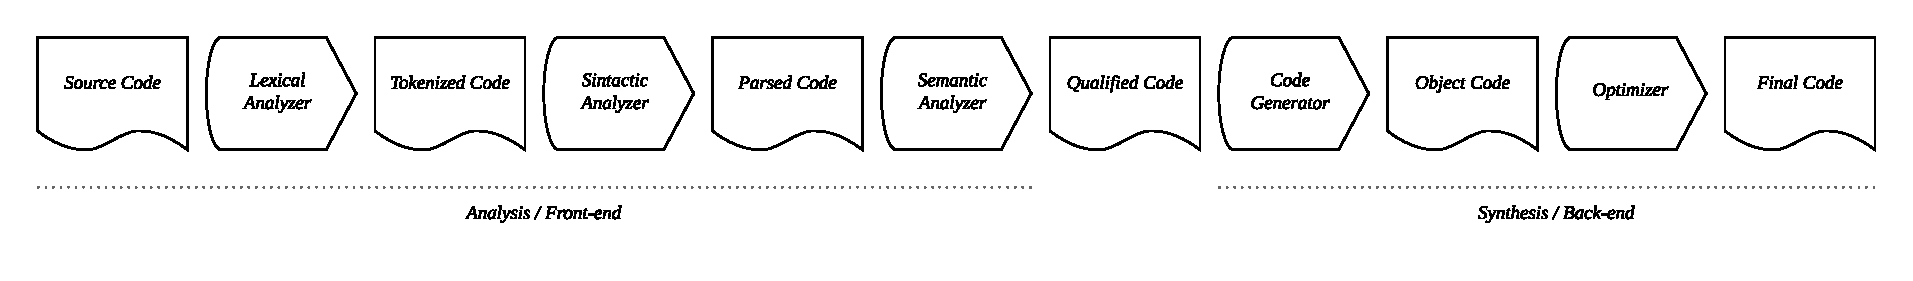
\includegraphics[width=50mm,scale=0.5]{compiler-stages}
  \caption[Compiler stages]{Compiler stages.}
  \labfig{compiler-stages}
\end{figure}

\subsubsection{Lexycal Analyzer}
The lexical analyzer task is to get the input and split it in to tokens \sidecite{lexical-analysis}, which are build from lexemes. If the compiler cannot find a valid token for some lexemes in the source code will generate an error, as the input cannot be recognized.

\subsubsection{Syntactic Analyzer}
The syntactic analyzer takes the tokens generated during the lexical analysis and parses them in such a way that try’s to group tokens so the conform to the language grammar rules. During this stage if there is any error while trying to group the tokens then the compiler will rise an error as the input cannot be parsed.

\subsubsection{Semantic Analyzer}
The semantic analyzer has two main tasks, usually. First it validates that the source code semantics are correct, for example 4 + “aaa” would not make sense. And the second task is to transform the Abstract Syntax Tree in to a type-checked and annotated AST. Usually that means relate the invocations and variables to its definition, very useful for type-checking.

\subsubsection{Code Generator}
The task of the code generator as its name indicates is to generate the target code, it can be byte code, machine code or even another high-language code.

\subsubsection{Code Optimizer}
The code optimizer is the last step before the final target code is generated, it rewrites the code that the code generator produced without changing the semantics of the program, its aim is just to make code faster. At \sidecite{compiler-optimizations} you can see an example of some optimizations that can be done at compile time to make your code faster.

\subsection{Conventional Compilers}
Conventional compiler are a big monolith where each stage \reffig{compiler-stages} is executed automatically after the previous stage, if the compiler has eight steps you need to execute them all at once. This approach have been the “old-fashion” but it presents some drawbacks:
\begin{itemize}
	\item A poor IDE \sidecite{ide} integration. IDE’s need to perform incremental compilations in matter of nanoseconds so the user doesn’t feel lag when typing the program. With conventional compilers as you need to go through all the compilation process at once they where very slow and companies like Microsoft need to develop different compilers, one for the IDE and another for the final compilation of the program itself. This lead to several problems like that if a feature gets implemented in the final compilation compiler but not in the IDE one the IDE would not support the feature meanwhile the language would.
	\item Difficult to debug. As the conventional compilers where a blackbox the only way to test intermediate stages was by throwing an input and waiting the the feature you wanted to test was thrown for that input.
\end{itemize}

\subsection{Modern Compilers}
After the problems Microsoft had with the C\# compiler they decide to rewrite the whole compiler and introduce a concept called “compiler as an API” with Roslyn \sidecite{dotNet}. This concept has been perfectly accepted and solved many problems. In this concept each stage has an input and an output that can be accessed from outside the compiler and stages can be executed independently on demand. This means that for example if an IDE just want to execute the Lexer the Parser and the Semantic analysis it can. That translates in to speed for the user.

Also the second problem is solved as testing individual parts of the compiler is much more easy than the hole compiler at once.


\setchapterpreamble[u]{\margintoc}
\chapter{Related Work}
\labch{related-work}

Some work has already been done in the field of Shape Expressions and RDF validation technologies. In this chapter we will go overthe main studies related to our project, exploring what they have achieved and someof their limitations.

% Section 1, Simplifications of shex.
\section{Simplifications of ShEx}
\labsec{ch03-shex-simplifications}

\subsection{The \textbf{S} language}

In 2019 at \sidecite{rdf-challenges} was defined a language called \textbf{S} as a simple abstract language that captures both the essence of ShEx and SHACL. This is very relevant as this language is intended to be the input of a theoretical abstract machine that will be used for graph validation for both ShEx and SHACL. Also in the same paper the authors carefully describe the algorithm for the translation from ShEx to S and from SHACL to S.

Although the theoretical abstract machine has not been implemented yet the intention of the WESO Research Group, where this S language was defined, is to devote more efforts in to this project during the 2021.

Other definition of an abstract language based on uniform schemas can be found at \sidecite{iovka-auto-shex-shacl}. This language is focused on schemas inference rather on validation, but needs to be taken into account as they also perform an abstraction of both ShEx and SHACL.

And to the best of our knowledge and after the research process carried out for this project no other language based on a subset of Shape Expressions has been designed nor implemented yet.

\subsection{ShEx Micro Spec}

% Section 2, ShEx ecosystem tools.
\section{ShEx Ecosystem Tools}
\labsec{ch03-shex-ecosystem}

We already know that ShEx and SHACL have been the two main technologies for RDF validation and some tools emerged around them, we thinks that some of them might benefit from ShEx-Lite. Here we introduce briefly those that had the biggest impact in the community.

\subsection{Validators}
Since the beginning of ShEx and SHACL as languages the RDF community started to build tools that take as input the schemas defined and validate graphs.

This kind of tools can benefit from SHEx-Lite from the point of view that new functionalities can be easily implemented and tested in the lite version of the language before even touching the stable releases of both tools. In the case of ShEx this is more obvious as ShEx-Lite and ShEx are both implemented in Scala and if good design principles are used functionalities can be just migrated and expanded for the rest of the language.

The most important validators are:

\subsubsection{Shaclex}
According to the Shaclex\sidenote{\url{https://github.com/weso/shaclex}} official website it is an Open Source Scala pure functional implementation of an RDF Validator that supports both Shape Expressions and SHACL. It was initially developed by Dr. Jose Emilio Labra Gayo and is being maintained by an active community on GitHub. It is used by different projects around the globe and its goal is to validate RDF graphs against schemas defined in Shape Expression or in SHACL.
This implementation of a ShEx validator is very important for us as ShEx-Lite is completly inspired by it and aims to transfer the sintactic an semantic validation enhancements to it.

\subsubsection{ShEx.js}
Another example of os a ShEx validator implementation is \texttt{ShEx.js} which is JavaScript based and also open source on GitHub. This implementation is very important for the ShEx community as they defined the serialization of the AST in this implementation as the abstract syntax of ShEx.


\subsection{IDEs}
In order to facilitate the task of writing schemas some engineers decide to implement specific IDEs for the Shape Expressions Language.

This tools will completely benefit from ShEx-Lite and there are currently collaborations in process. At the time they work with Shaclex, which is structured as a conventional compiler, but with the API architecture of ShEx-Lite IDEs can access directly to the syntactic and semantic modules so features like advances coloring syntax or incremental compilation are available.

\subsubsection{YASHE}
YASHE\sidenote{\url{https://github.com/weso/YASHE}} (Yet Another ShEx Editor), is a Shape Expressions IDE which started as a fork ofYASQE(which is based on SPARQL). This tool performs lexical and syntactic analysis of the content of the editor, thus offering the user a realtime syntactic error detector. It has features like: syntax highlighting, visual aid elements (tooltips) and autocomplete mechanisms. In addition, it offers a simple way of integrating into other projects.

\subsubsection{Protégé}
Protégé is a piece of software developed by the University of Stanford focused on ontology edition. During the last year they added support for Shape Expressions dition on their own software so they became another ShEx IDE.

\subsubsection{VSCode}
VSCode is a source code light-weight editor developed by Micorsoft and supported by Linux, macOS and Windows. By default this editor does not support any programming language, the way it works is with packages that the community develops and extends the functionality. One of those packages adds support for Shape Expressions Compact syntax and transforms VSCode into a ShEx IDE.
This plugin does not add semantic validation and it is a clear target to benefit from ShEx-Lite features.

\subsection{Others}
Other researches focused their efforts in to inferring schemas to existing data sets and creating tools to that evolved from ShEx in order to transform existing data.

\subsubsection{Shexer}
Shexer\sidenote{\url{https://github.com/DaniFdezAlvarez/shexer}} is a python library aimed to perform automatic automatic extraction of schemas in both ShEx and SHACL from an RDF input graph. That is if all the other tools take the schemas as the input and validate a graph with it, this tool takes a graph and from it it infers the schemas that it might contain. Its work is fully described in \sidecite{iovka-auto-shex-shacl, fernandez2016inference}.

\subsubsection{ShExML}
ShExML\sidenote{\url{https://github.com/herminiogg/ShExML}} is a language based on ShEx (not a simplification nor an abstraction of ShEx) that can map and merge heterogeneous data formats into a single RDF representation. The main idea behind this tool is written at \sidecite{shexml}.

\bigskip

An example of how this different tools can work together thanks to ShEx-Lite would be the following, illustrated at \reffig{shex-lite-shexer-integration}.
Wikidata currently holds millions of registers that do not have any schema that validates them. And they need to make consumer that represents the data in to an object domain model. Without any tool this is just almost impossible, but this shexer you can infer the schemas to ShEx-Lite syntax and with the ShEx-Lite compiler you can automatically create the object domain model in your favorite OOL.

\begin{figure*}[h!]
	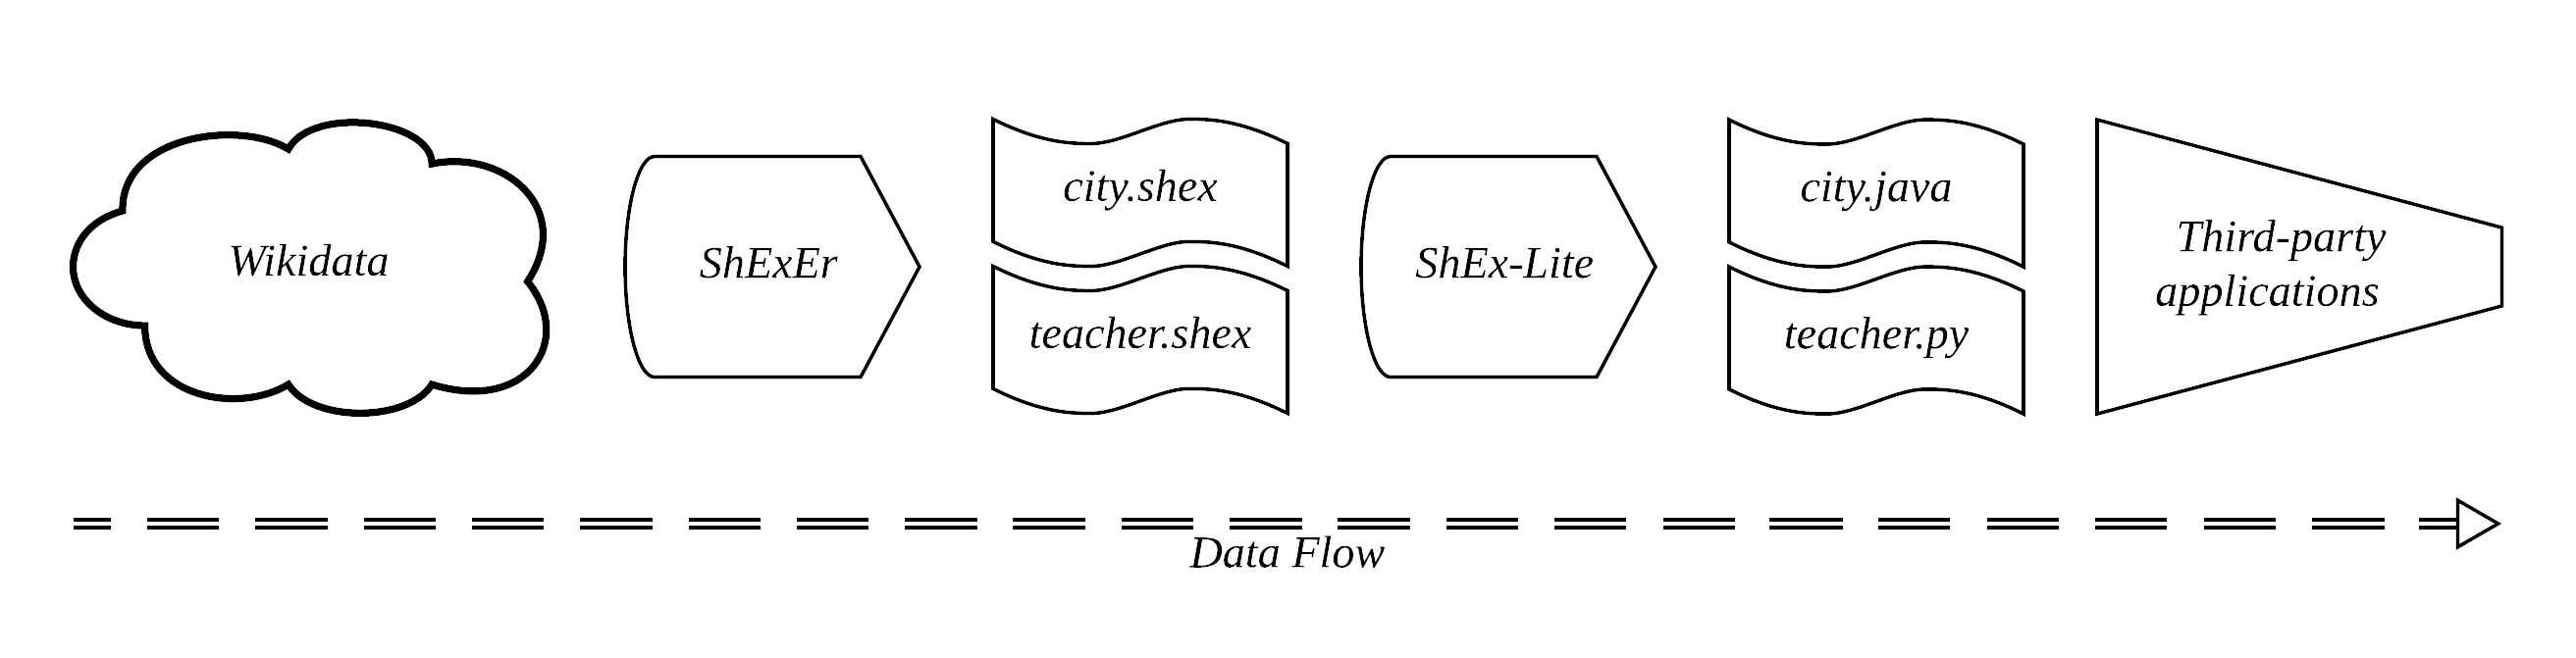
\includegraphics{shex-lite-shexer-integration}
	\caption[ShEx-Lite integration with Shexer]{ShEx-Lite integration with Shexer for automatically generating java domain object models for the Wikidata schemaless existing data. This shoes the schemaless data from wikidata from which shape expressions are infeered by shexer and later transformed to java plain objects by means of ShEx-Lite so third party apllications can implement the domain model.}
	\labfig{shex-lite-shexer-integration}
\end{figure*}
\setchapterpreamble[u]{\margintoc}
\chapter{System Analysis}
\labch{system-analysis}

In this chapter we present the analysis that was carried out in order to design the compiler. First we sumarize the objectives and the target users of the compiler, this will be the starting point of the analysis. After, we will define an scope from which we will stract the use cases and requirements that, finally, will help to identify possible subsystems for the design phase, explained in \refch{system-design}.

\section{Objectives}
\labsec{ch04-objectives}

The objectives are those results that we want to achieve or features that we want the compiler to have once it is implemented. The main objectives that we have identified for the compiler are the following ones:
\begin{itemize}
    \item Provide the following tools from the compiler:
    \begin{itemize}
        \item Get the ST (syntax tree) from a source file.
        \item Get the AST (abstract syntax tree) from a ST.
        \item Get the SIL (ShEx-Lite Intermediate Language) from an AST.
        \item Generate sources in a given OOL from a SIL.
        \item For all the previos functionalities detect and inform or any event considered by the compiler as an error or warning.
    \end{itemize}
    \item Natively support, at least, Java and Python as target languages for the code generation.
    \item Allow the previous tools to be called from CLI.
    \item Allow the previous tools to be encapsulated in other programs written in any Java based language.
    \item Include examples of how the compiler works with a representative set of shape expressions.
\end{itemize}

\section{Target Users}
\labsec{ch04-target-users}

Every system has some target users, in the case of the SeX-Lite compiler we will focus it on three different types of users:
\begin{itemize}
    \item People with low technical skills that want to make schemas to validate RDF by means
    of shape expressions. This people will be able to compile their schemes and check for
    syntax / semantic errors or warnings through the CLI with a very simple instruction set.
    \item People with medium technical skills that want to transform a set of shape expressions
    in to a domain object model automatically. For this people the compiler will provide a
    manual that will explain each step of the transformation and an usage example.
    \item ShEx Community developers that want to test a new feature by implementing and
    testing its behaviors in a controlled small environment. For this people the compiler
    provides not only the public API but the source code and the corresponding technical
    documentation. 
\end{itemize}

\section{Use Cases}
\labsec{ch04-use-cases}

The first stage to analyze our system is to see the use cases view, from there we will try to capture posible requirements and with all that information design our system.

\begin{figure}[hb]
    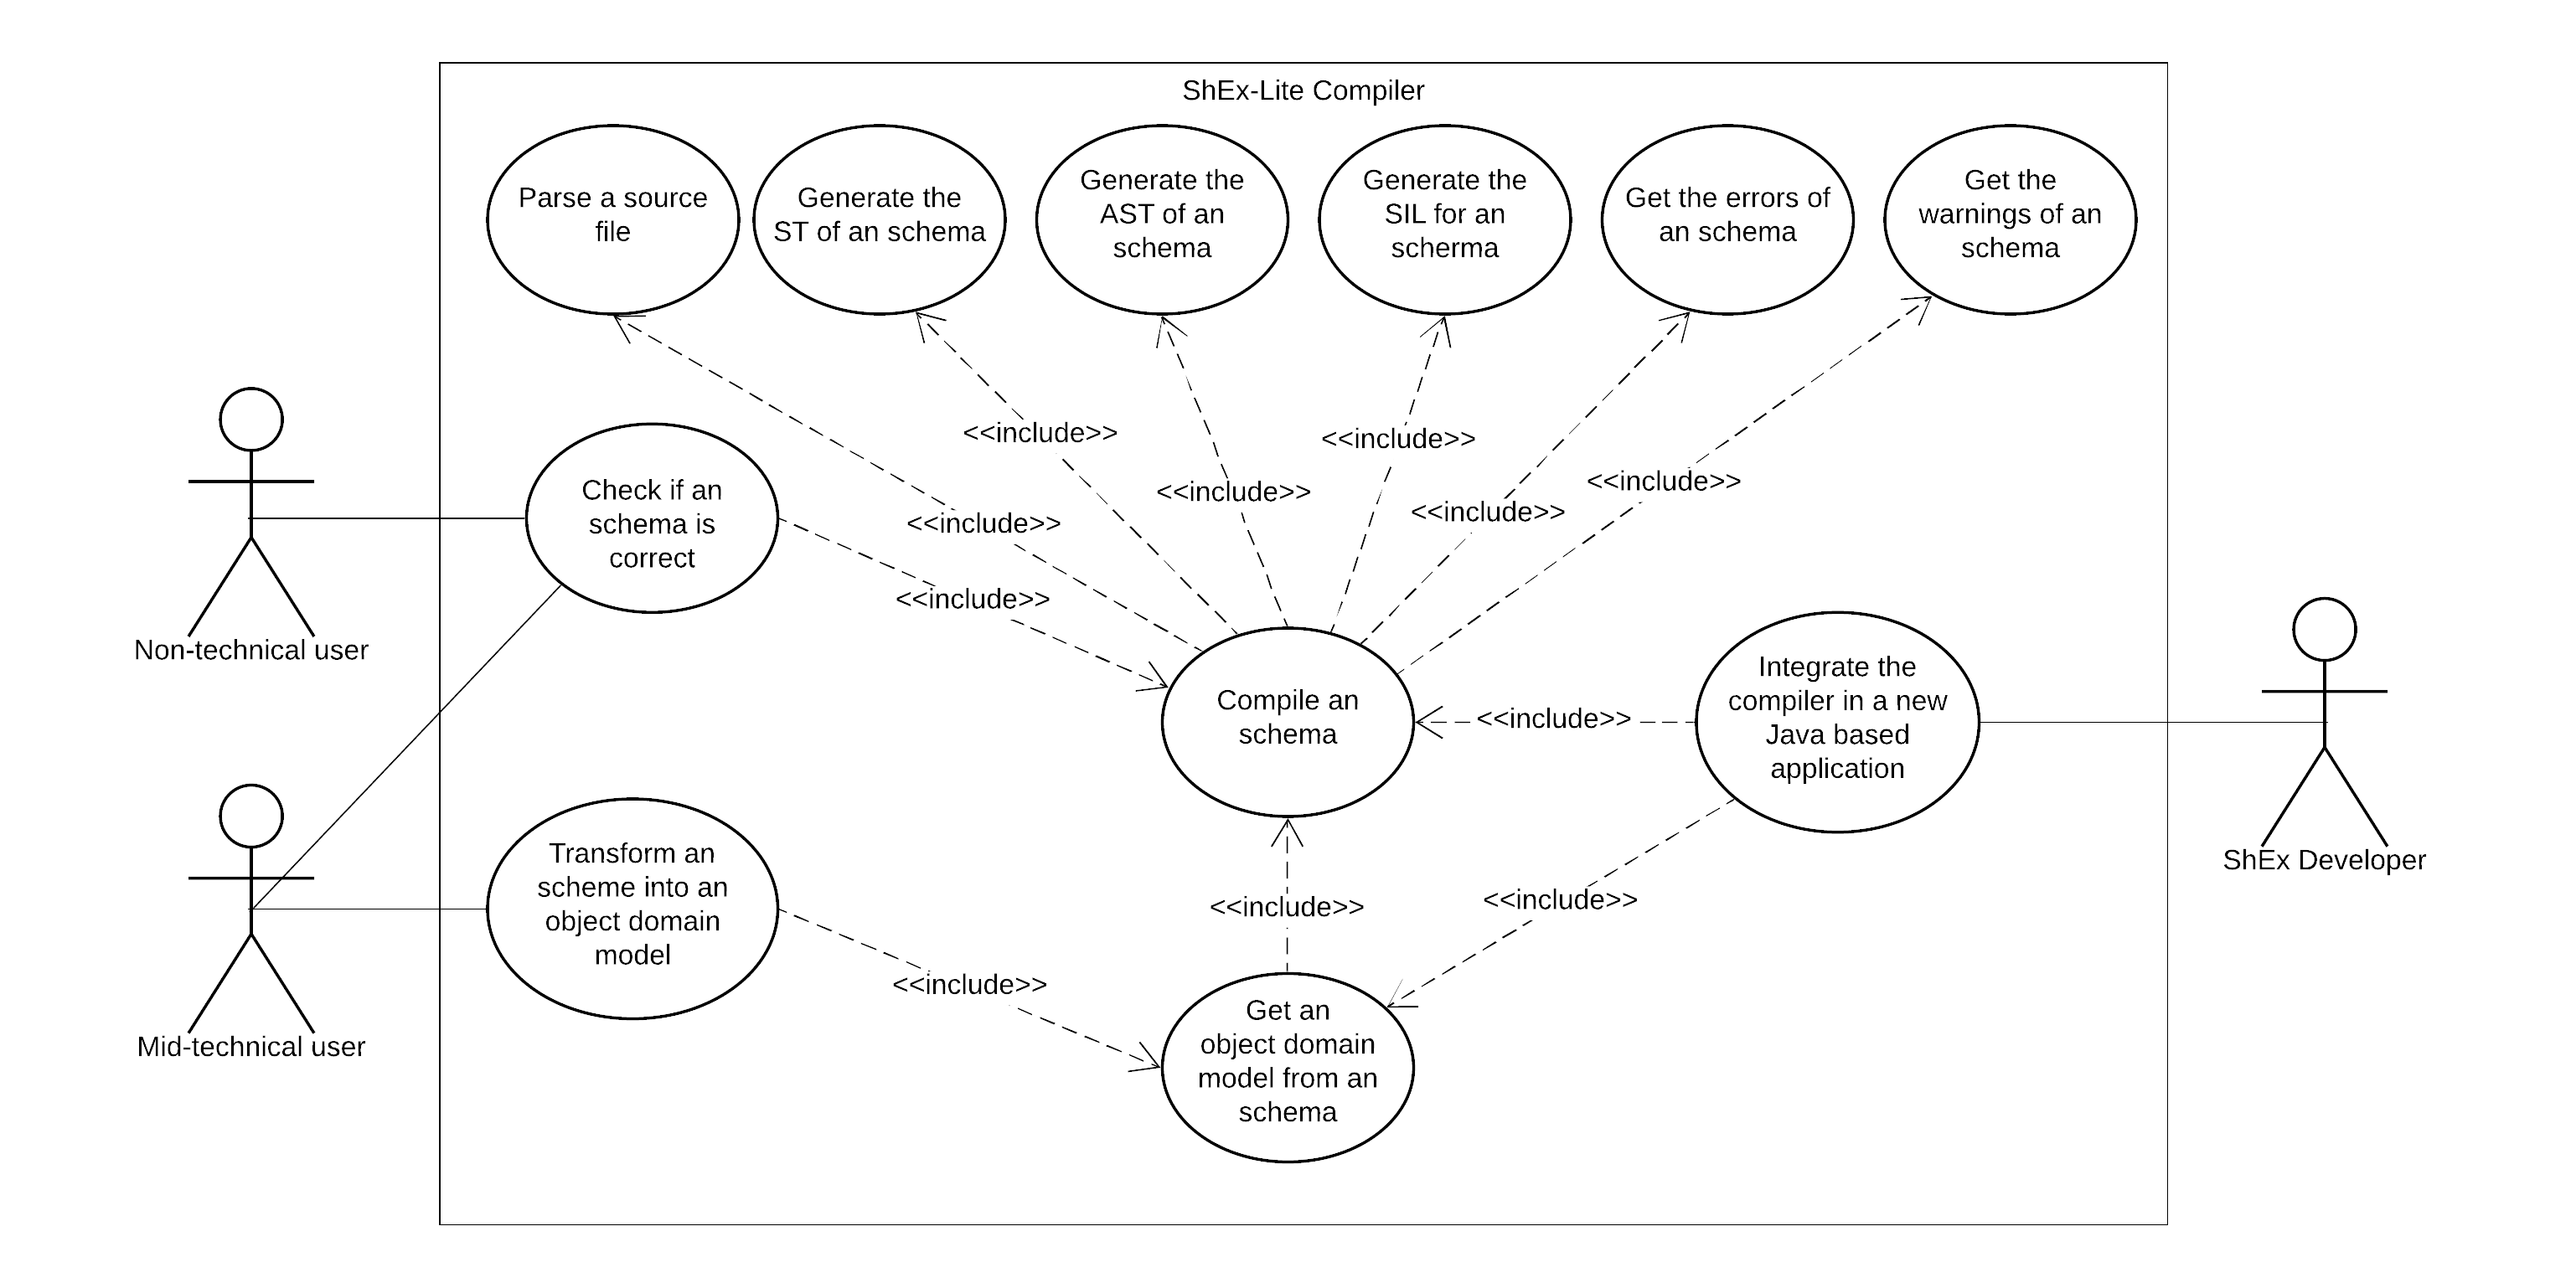
\includegraphics{shex-lite-use-cases-01.png}
    \caption[Use cases view of the ShEx-Lite compiler for the three different actors of the system]{Use cases view of the ShEx-Lite compiler for the three different actors of the system.}
    \labfig{shex-lite-use-cases-01}
\end{figure}

In \reffig{shex-lite-use-cases-01} we can see the high level view of the different use cases that the three different target users of the systems might have, now we will analyze each one individually, some the internal use cases that have no direct interaction with the target user will be explored after.

\subsection{Non technical user}
The non technical target user is intended to use only the compiler to validate if the schemas they have defined are syntactically and semantically correct, or if they have any error or warning to be aware of them. \reffig{shex-lite-use-cases-02} shows the interaction diagram for this actor, and \reftab{use-case-01-tab} describes the represented use case.

\begin{figure}[hb]
    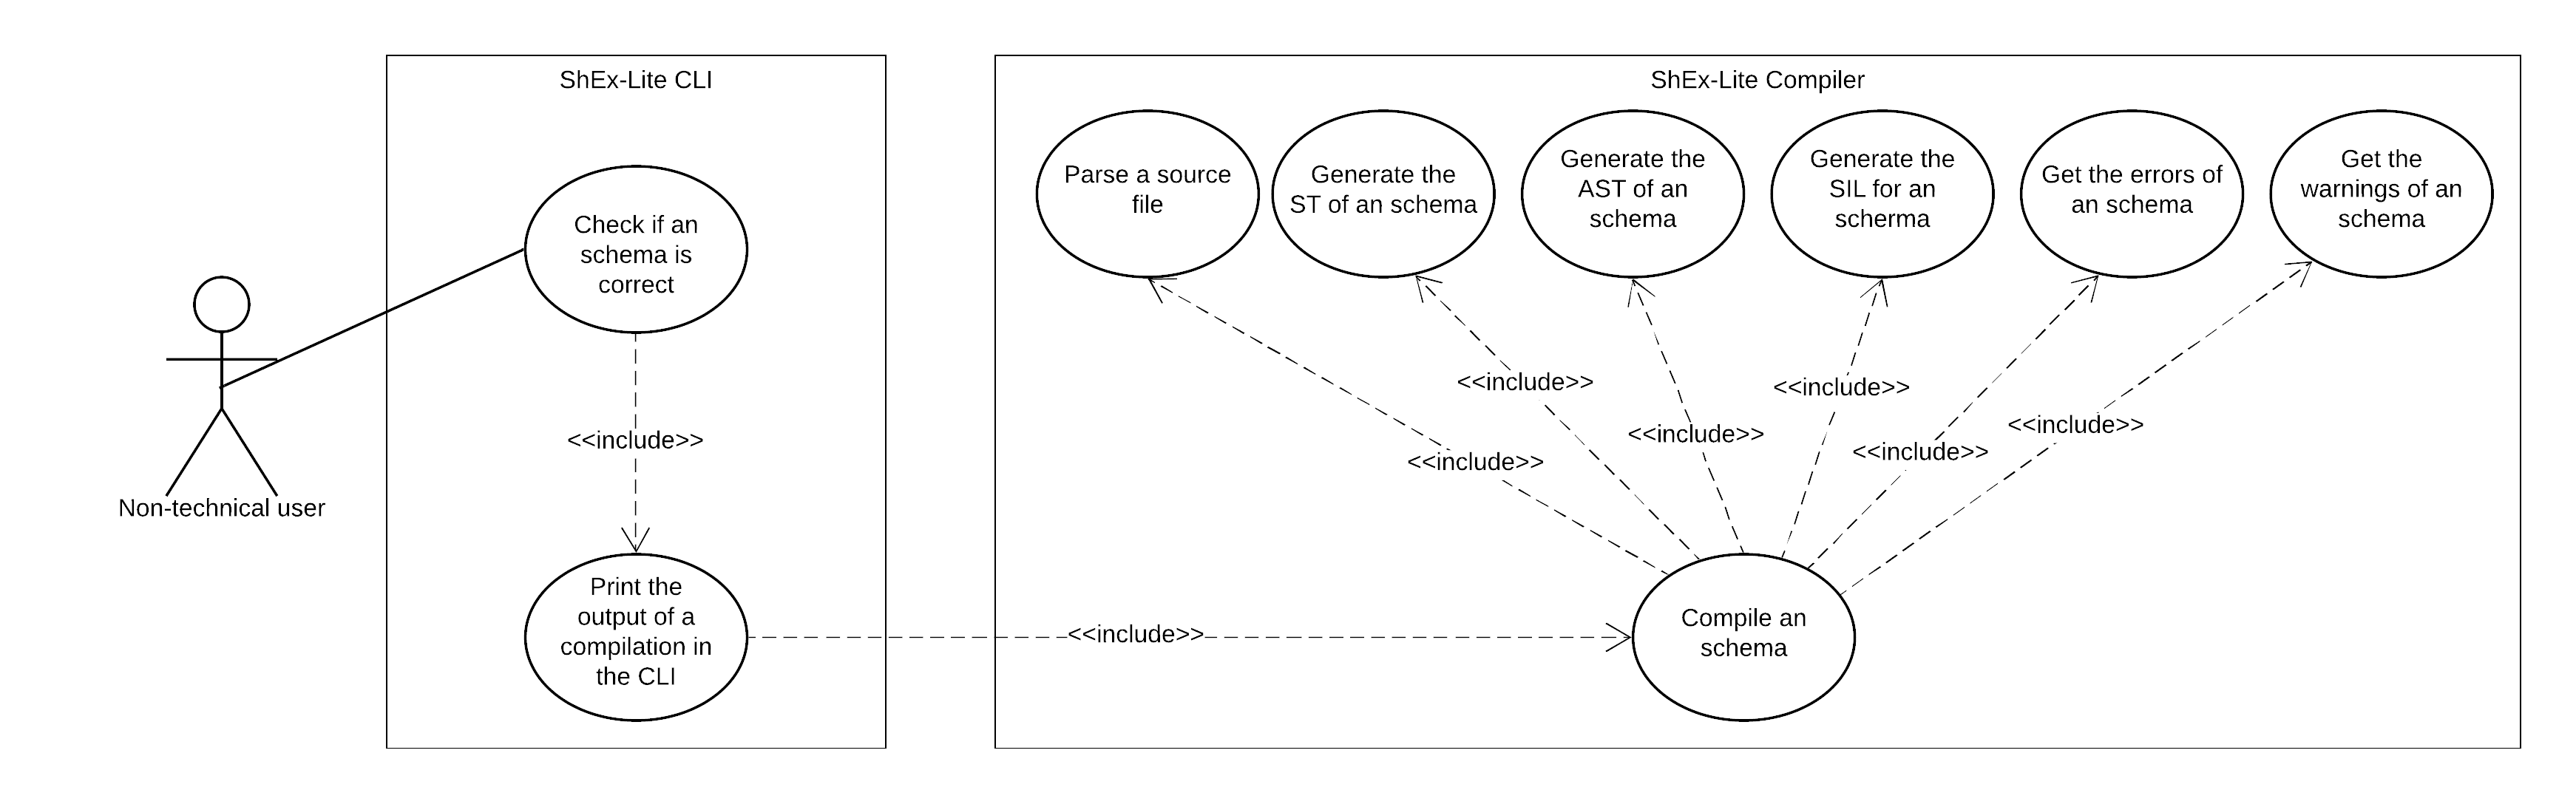
\includegraphics{shex-lite-use-cases-02.png}
    \caption[Extension of the use case view for a non technical user]{Extension of the use case view for a non technical user.}
    \labfig{shex-lite-use-cases-02}
\end{figure}

\begin{table}
    \begin{tabular}{ | m{2cm} | m{8cm}| }
        \toprule
        Use Case Number & 1 \\
        \midrule
        Description & Check if an schema is correct from the CLI tool. \\
        \midrule
        Actor & Non technical user. \\
        \midrule
        Flow & The actor wants to check if schema is correct or not. If it is not correct wants to see all the warnings / errors. For this purpose the actor introduces the schema in the CLI tool and starts the flow. Once the flow is complete the actor wants to see information that helps to decide if the schema is correct or not. \\
        \bottomrule
    \end{tabular}
    \caption[Definition of the use case number 1 for the non technical user]{Definition of the use case number 1 for the non technical user.}
    \labtab{use-case-01-tab}
\end{table}

\subsection{Mid technical user}
The use cases expected for a mid technical user are two, in one side the compilation in order to validate if their schemas are syntactically and semantically correct, or if they have any error or warning. And on the other hand, automatically generate the domain object models for the defined schema. For this user we can find the representation of the interaction diagram at \reffig{shex-lite-use-cases-03} and both associated use cases descriptions on \reftab{use-case-02-tab} and \reftab{use-case-03-tab}.

\begin{figure}[hb]
    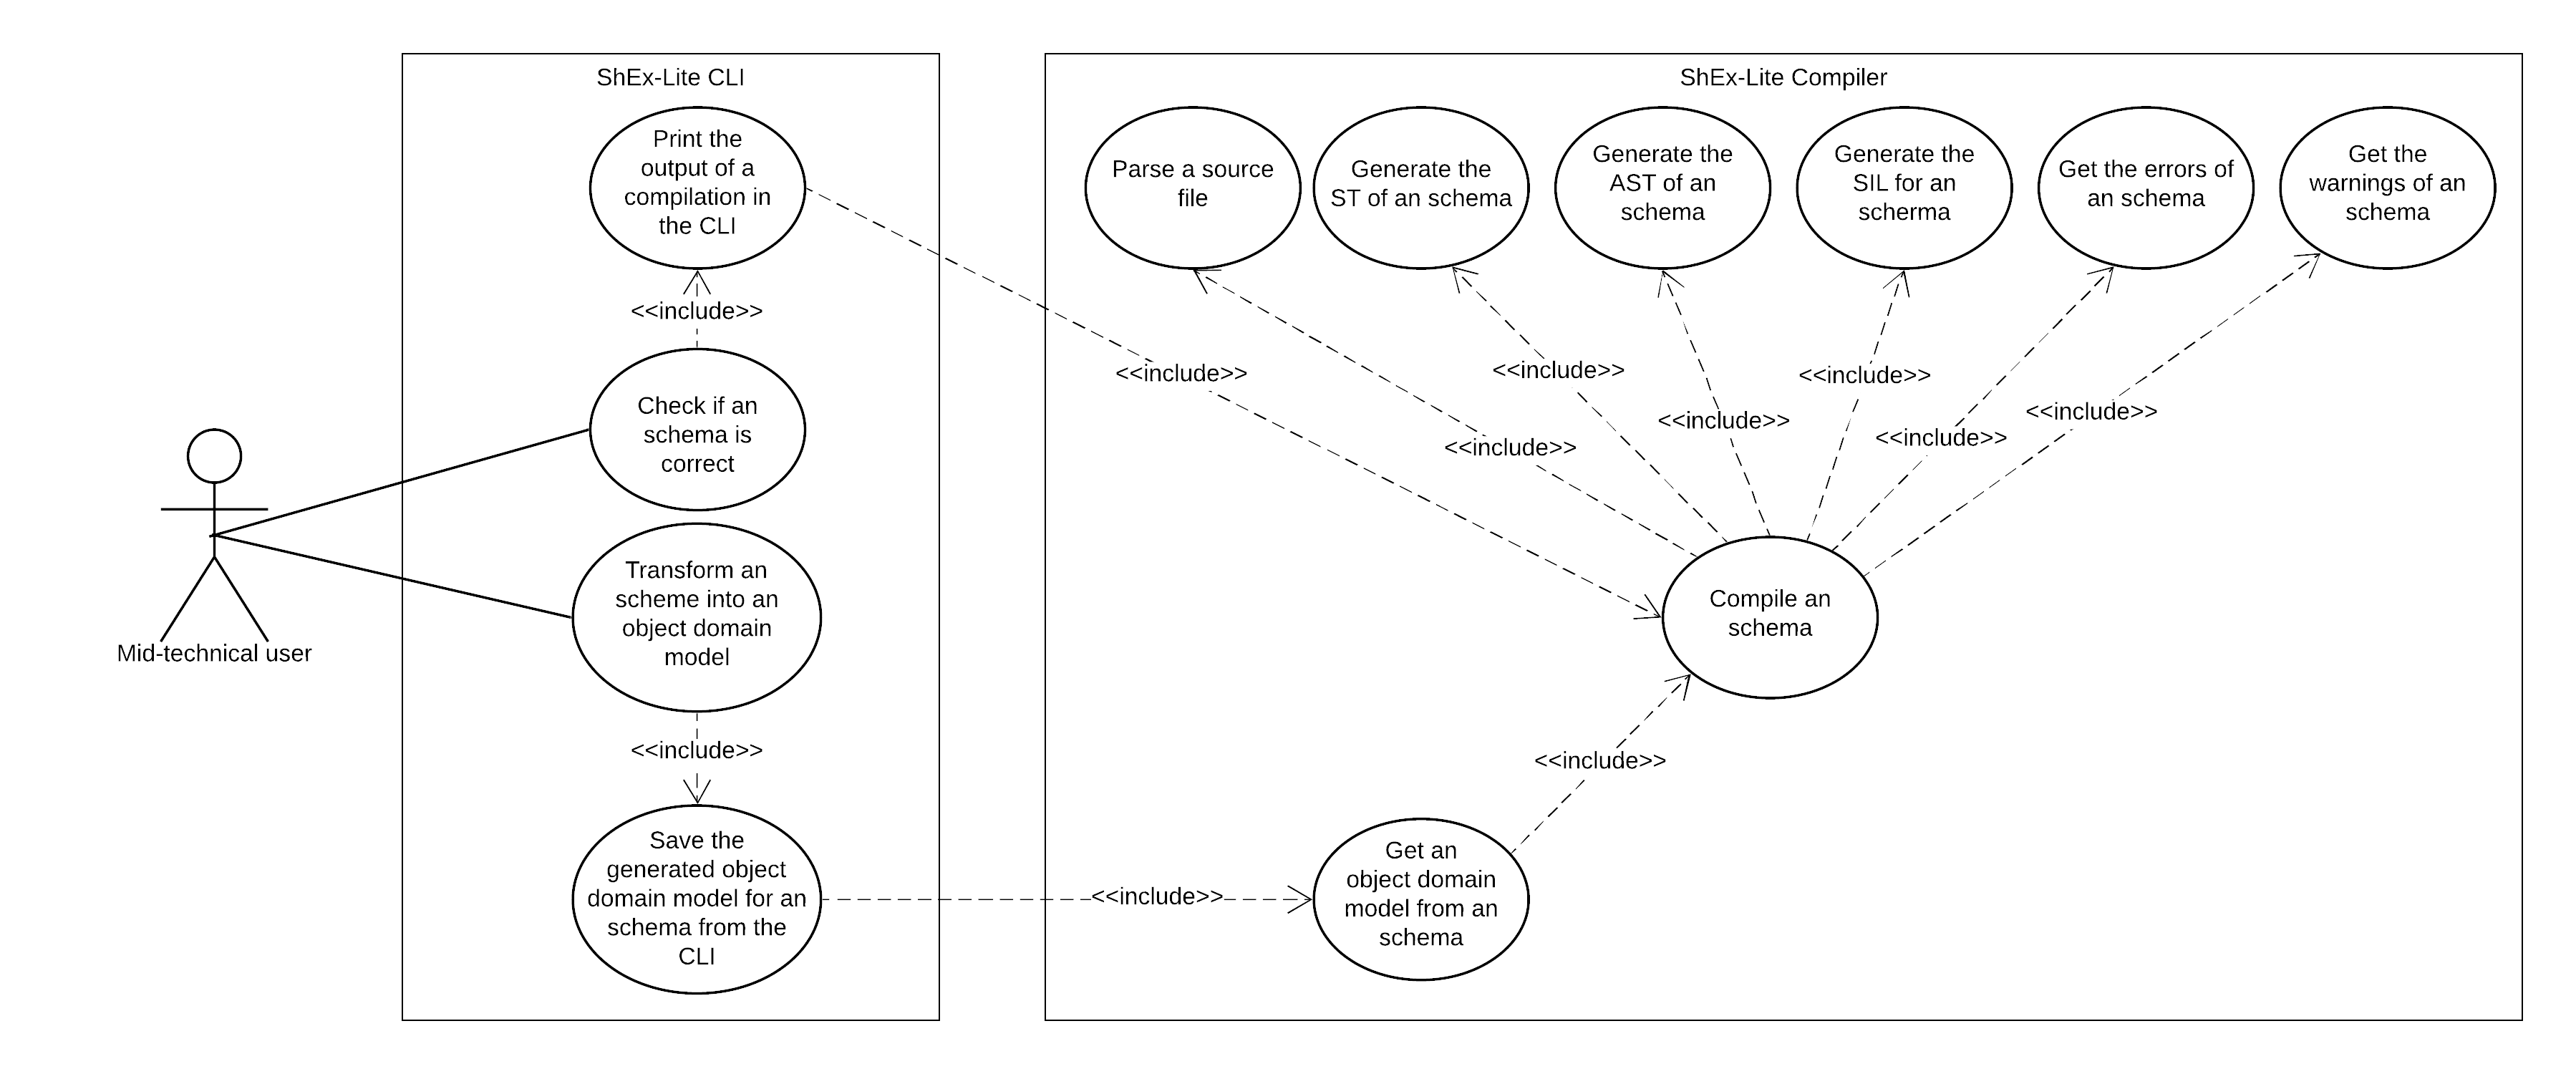
\includegraphics{shex-lite-use-cases-03.png}
    \caption[Extension of the use case view for a mid technical user]{Extension of the use case view for a mid technical user.}
    \labfig{shex-lite-use-cases-03}
\end{figure}

\begin{table}
    \begin{tabular}{ | m{2cm} | m{8cm}| }
        \toprule
        Use Case Number & 2 \\
        \midrule
        Description & Generate an object domain model for a given schema from the CLI. \\
        \midrule
        Actor & Mid technical user. \\
        \midrule
        Flow & The actor wants to generate an object domain model for a given schema from the CLI tool. For this purpose the actor introduces the schema in the CLI tool and starts the flow. Once the flow in complete the actor wants the generated object model to be persist as source files on his computer. \\
        Conditions & For this flow to end correctly it is mandatory that the schema that the user uses to generate the domain object model is correct. \\
        \bottomrule
    \end{tabular}
    \caption[Definition of the use case number 2 for the mid technical user]{Definition of the use case number 2 for the mid technical user.}
    \labtab{use-case-02-tab}
\end{table}

\begin{table}
    \begin{tabular}{ | m{2cm} | m{8cm}| }
        \toprule
        Use Case Number & 3 \\
        \midrule
        Description & Check if an schema is correct from the CLI tool. \\
        \midrule
        Actor & Mid technical user. \\
        \midrule
        Flow & The actor wants to check if schema is correct or not. If it is not correct wants to see all the warnings / errors. For this purpose the actor introduces the schema in the CLI tool and starts the flow. Once the flow is complete the actor wants to see information that helps to decide if the schema is correct or not. \\
        \bottomrule
    \end{tabular}
    \caption[Definition of the use case number 3 for the mid technical user]{Definition of the use case number 3 for the mid technical user.}
    \labtab{use-case-03-tab}
\end{table}

\subsection{ShEx Developer}
A ShEx developer is expected to use the compiler in two ways, first to integrate it in to other applications and secondly to generate object domain models for a given schema but not from the CLI, from an API instead. \reffig{shex-lite-use-cases-04} shows the interaction diagram of this actor with the compiler and \reftab{use-case-04-tab} descrives this use case scenario.

\begin{figure}[hb]
    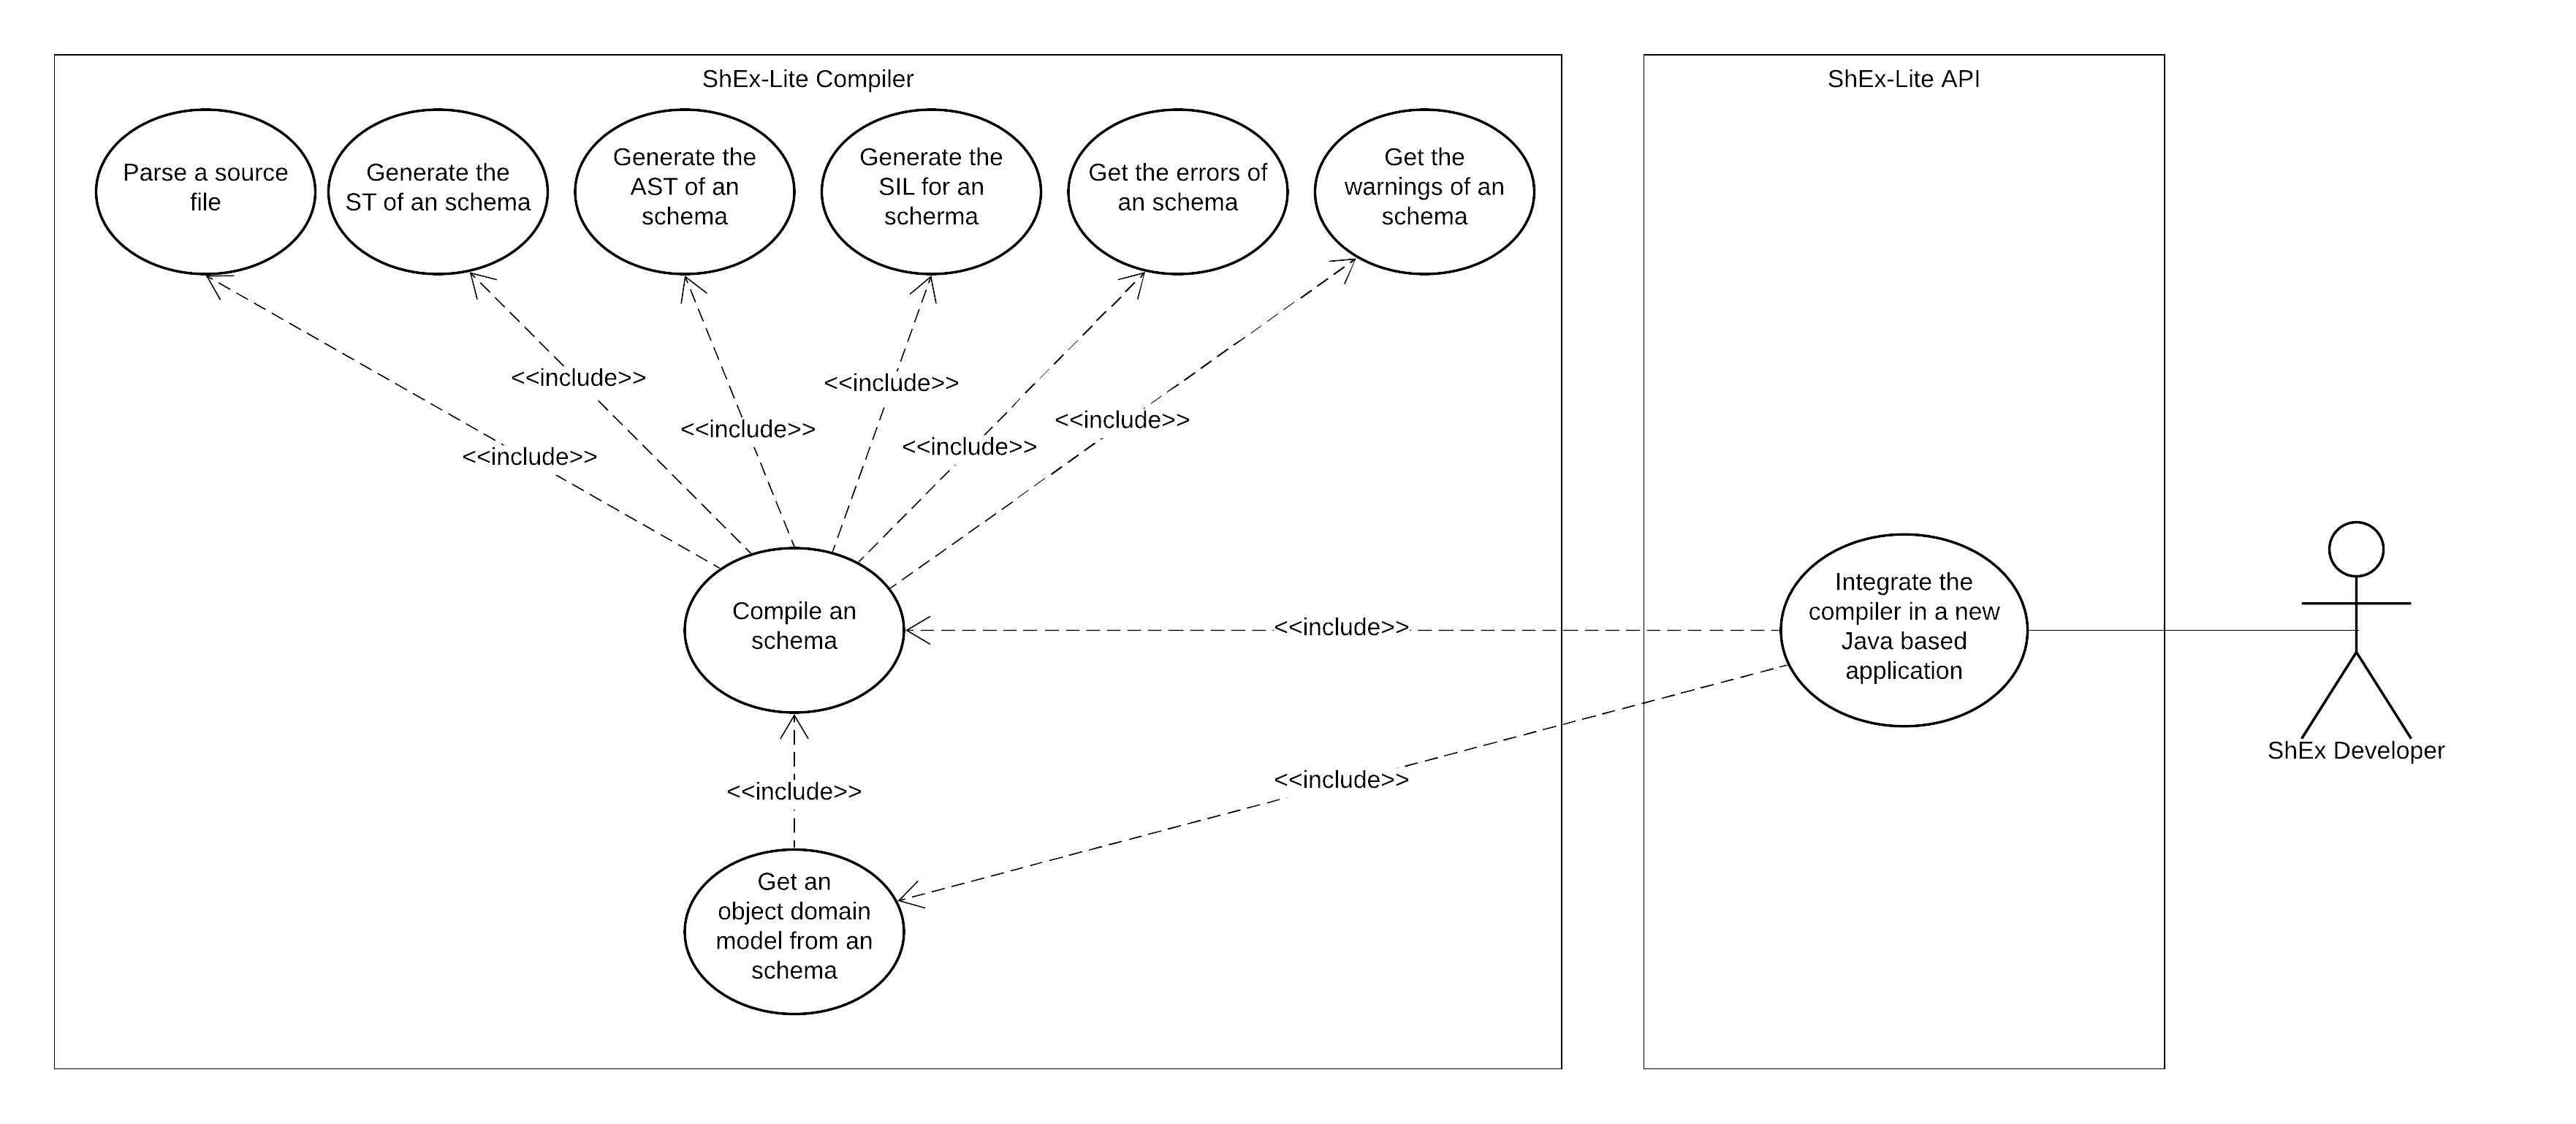
\includegraphics{shex-lite-use-cases-04.png}
    \caption[Extension of the use case view for a mid technical user]{Extension of the use case view for a mid technical user.}
    \labfig{shex-lite-use-cases-04}
\end{figure}

\begin{table}
    \begin{tabular}{ | m{2cm} | m{8cm}| }
        \toprule
        Use Case Number & 4 \\
        \midrule
        Description & Integrate the compiler in a new Java based application. \\
        \midrule
        Actor & ShEx developer. \\
        \midrule
        Flow & The actor wants to integrate the compiler in to a new java base application. For that purpose the actor will use a public API that allow the actor to integrate the actions described in the use cases 2 and 3. \\
        \bottomrule
    \end{tabular}
    \caption[Definition of the use case number 4 for the ShEx developer user]{Definition of the use case number 4 for the ShEx developer user.}
    \labtab{use-case-04-tab}
\end{table}

\bigskip
The previous use cases might seem like the system is really simple, but far from truth the
fact that the interface with the target users is simple does not define the complexity of the
system, as this, lives inside of it. In order to capture this complexity we will proceed now to
analyze the requirements that the implemented system must meet. 

\section{Requirements}
\labsec{ch04-requirements}

In this section we are going to enumerate the requirements that we have obtained for the
compiler. Since the line that separates functional and non-functional requirements can be
sometimes hard to define, we decided to specify the requirements following the taxonomy
introduced in the IEEE 830 standard for the specification of software requirements. The
following types of requirements will be evaluated:

\begin{itemize}
    \item External interfaces: Requirements that affect user, hardware, software or communication interfaces.
    \item Functional requirements: Requirements related to the functions of the system.
    \item Performance requirements: These requirements are related to the load that the system should tolerate.
    \item Logical database requirements: These requirements are related to access or constraints with the system’s database.
    \item Design constraints: Constraints imposed by standards, hardware limitations…
    \item Other constraints.
    \item System attributes: Quality attributes of the system, such as usability, accessibility…
    \item Other requirements that do not belong to any of the categories above.
\end{itemize}

\subsection{External Interfaces}

\subsection{Functional Requirements}

\subsection{Performance Requirements}

\subsection{Design Constraints}

\subsection{Other Constraints}

\subsection{System Attributes}

\subsection{Other Requirements}


%\section{Identified Subsystems}
\labsec{ch04-subsystems}

Once the definition of the scope was finished, and the requirements were captured and documented, the following subsystems were identified.

\subsection{Compiler}
The compiler subsystem, called shexlc includes all the necessary elements to validate that
an schema is correct, or provide with the necessary information to fix any error it might
contain. And generate domain object models for the correct schemas. 

\subsection{CLI tool}
The CLI Tool provide both non technical and mid technical users the ability to use the
compiler from a text interface, allowing them to validate syntactically and semantically the
schemas. This validation involves also informing if any error or warning is generated during
the compilation. And in the case mid technical users also it provides the ability to generate
domain object models by saving them in the computer as source files. 

\subsection{Public API}
The compiler public API, called shexl, provides to the ShEx Community developers the
ability to access the different stages of the compilation process independently. Its main
objective is to provide them with a simple API that allows them not only to integrate the
compiler on different applications but also to extend it easily. 
\setchapterpreamble[u]{\margintoc}
\chapter{System Design}
\labch{system-design}

In this section we will explore que design of ShEx-Lite language and compiler,
from the most general diagram to a deeper level that gives a clear idea of the
architecture of ShEx-Lite compiler.

\section{ShEx-Lite Language Design}
\labsec{ch05-language-design}

In the previous section we just seen the analysis of the requirements for the
syntax that we will develop in next chapter, here, in this section, we will
design the syntax from an abstract point of view.

The requirements alredy left preaty clear the functionalities of the language,
it must allow to \textbf{define prefixes}, \textbf{define a base}, \textbf{define the start shape expression}
and to \textbf{define shape expressions}. Therefore our languge will be formed by a set of definitions.

It is very important aso, in order to meet the quality attributes, that our syntax is based on Shape Expressions
Compact Syntax. That means that if our syntax is an extrictly subset of \texttt{ShExC} the systems that already
work with ShEx will work with ShEx-Lite. This has been disccused in \sidenote{\url{https://github.com/weso/shex-lite-evolution/pull/1}}.

\subsection{Prefix Definition}
The prefix definition will follow the same specification as in ShEx, that means that will assign an IRI to an String Identifier.
In ShEx it is allowed to re-assign a new IRI value to an existing identifier prefix \textit{(also called prefix overrdide)},
but in ShEx-Lite, as it is horiented to users with lower technical skills, this is not allowed.
This way we improve the safety of the language and its discussion can be found in \sidenote{\url{https://github.com/weso/shex-lite-evolution/pull/16}}.

In \texttt{ShExC} the prefix definition is representented by the keyword \texttt{prefix} followed by the string identifier, which can
be empty, then the colon symbol and finally the IRI. Therefore the production would be:

\begin{center}
    \begin{verbatim}
PrefixDefinition :: 'PREFIX'  ID ':' IRI
    \end{verbatim}
\end{center}

\subsection{Base Definition}
The base definition defines the IRI that will be use as base for other relative IRIs that could appear in the schema. By default the base
already contains an IRI that points to a default location and it is allowed to declare only one base definition in the schema. This is also done
by safety and its discussion can be found in \sidenote{\url{https://github.com/weso/shex-lite-evolution/pull/16}}.

Also we will inherit the \texttt{ShExC} syntax and the base definition will have the following production:

\begin{center}
    \begin{verbatim}
BaseDefinition :: 'BASE' IRI
    \end{verbatim}
\end{center}

\subsection{Start Definition}
The start definition does not have any implication within an scheme, its functionality is to indicate at validation time the default shape expression to use
if no other shapoe is indicated. As a difference with ShEx and in order to increase language safety we do not allow the start declaration to appear more than once.
This is an open discussion in ShEx community, the start shape expression that it is used is only the last one defined and the definition has no functionality during
compilation therefore if two start definitions appear the first one is like it never existed.

We will also folloe the \texttt{ShExC} syntax for this element and its production will be:

\begin{center}
    \begin{verbatim}
StartDefinition :: 'START' '=' ShapeReference
    \end{verbatim}
\end{center}

The \textit{ShapeDefinition} production also includes another rule that is the \textit{ShapeReference}. This rule production is not important at thi point,
but the important part is that it represents a reference to a shape expression definition that must be defined within the schema, at any possition.

\subsection{Shape Expression Definition}
The final element of the definitions is the Shape Definition, a shape definition is defined as a set of triple expressions, where each triple
expression is formed by the \textit{property}, the \textit{constraint} and the \textit{cardinality}. In ShEx this element definition is much more
complex, allowing logical operation between triple expressions and even assignments. In our case we simplified this element to cover the needs described
during the analysis. Our production for Shape Definition would be:

\begin{center}
    \begin{verbatim}
ShapeDefinition :: ShapeIdentifier '{' TripleExpression+ '}'
    \end{verbatim}
\end{center}

Notice the \textit{ShapeDefinition} contains a \textit{ShapeIdentifier}, this identifier is another prodsuction and at the end it is an IRI, it must
be unique in the schema and it stores the non-empty set \textit{(represented by the + symbol)} of triple expressions.
\section{Architecture}
\labsec{ch05-architecture}
There were several elements that conditioned the architecture of this system. First of all,
there is no database or data access layer that needs to be taken into account. There isn’t
also any presentation or visual interface of data other from the CLI. The system consists
mainly of functionality that is offered to other users to use from the CLI or create their own
systems. 

All of these elements simplified noticeably the architecture of the system. \reffig{shex-lite-high-level-arch} sumarizes the high level architecture of the ShEx-Lite compiler. Notice that the elements that appear here are the same that where identified in \refch{compiler-analysis}.

\begin{figure}[hb]
    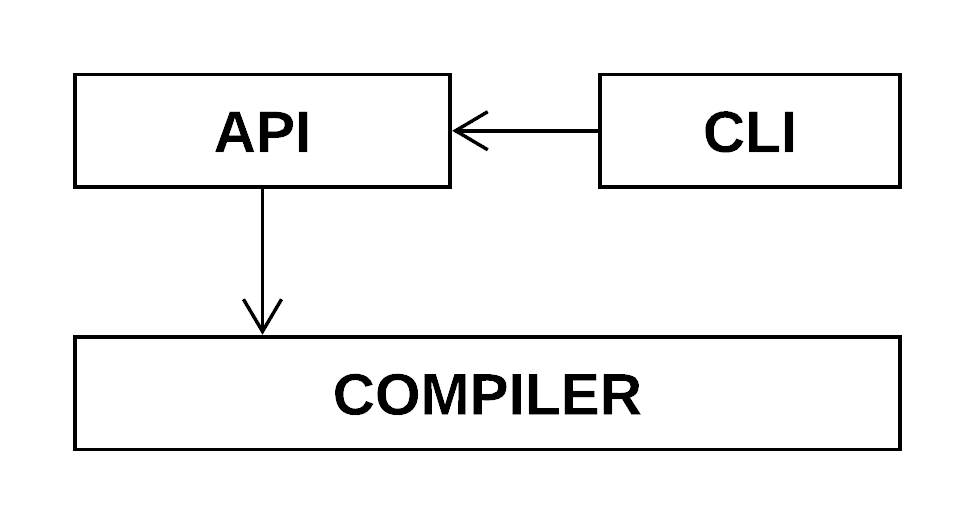
\includegraphics{shex-lite-high-level-arch.png}
    \caption[High level view of the ShEx-Lite system]{High level view of the ShEx-Lite system. This figure shows how the CLI is build on top of the API which depends on the compiler implementation.}
    \labfig{shex-lite-high-level-arch}
\end{figure}

\begin{figure}[hb]
    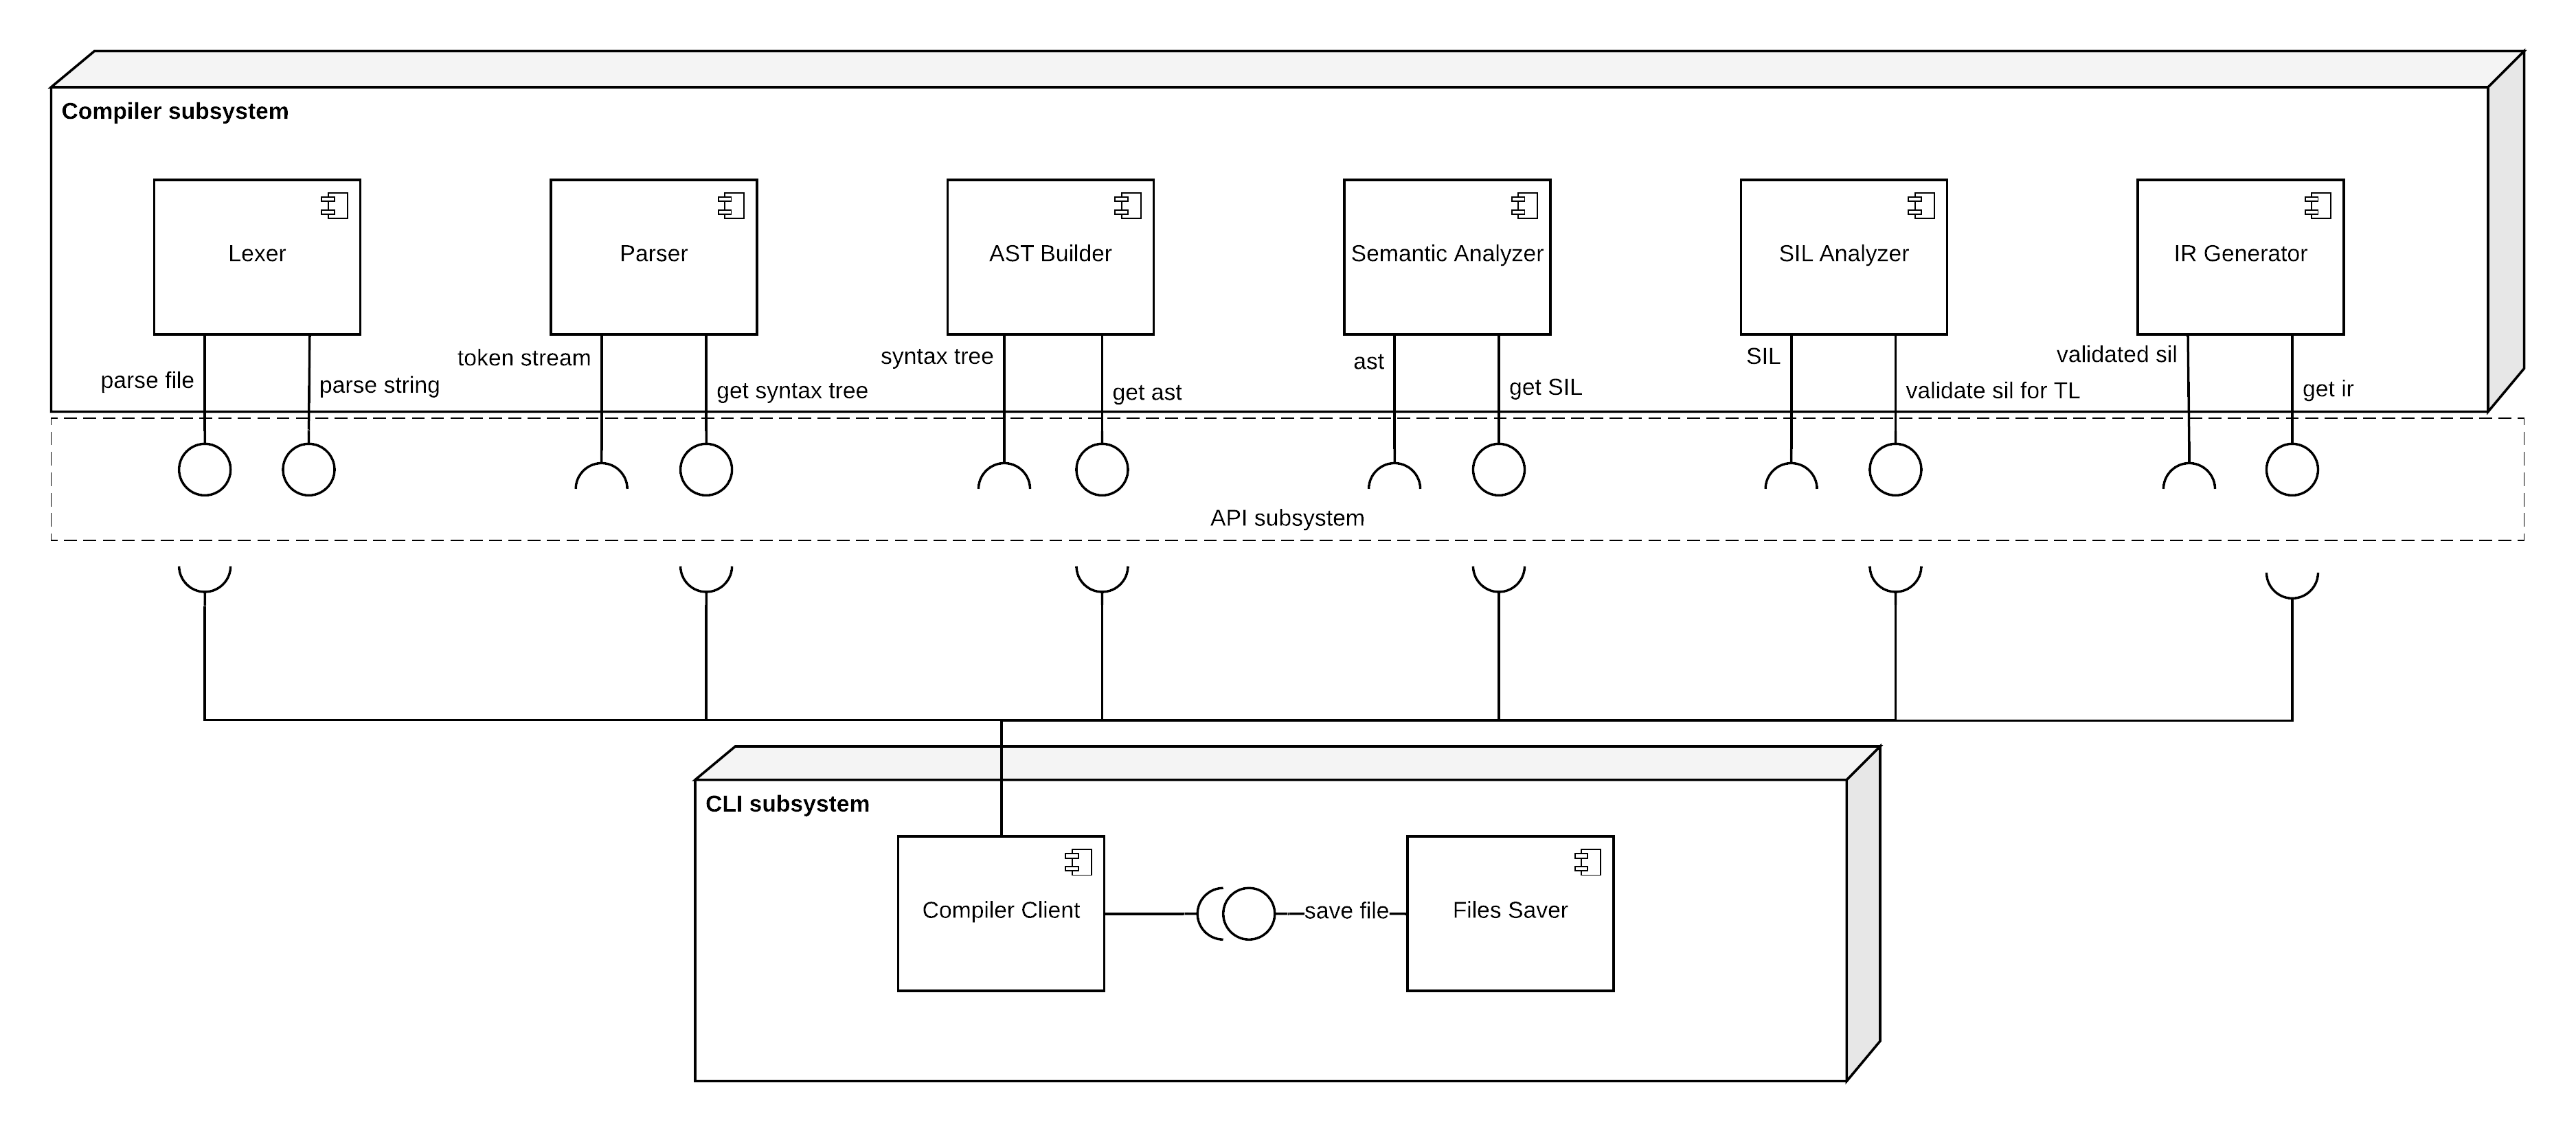
\includegraphics{shex-lite-components.png}
    \caption[Components diagram for ShEx-Lite Compiler]{Components diagram for ShEx-Lite Compiler.}
    \labfig{shex-lite-components}
\end{figure}

\reffig{shex-lite-components} shows the three main subsystems that the ShEx-Lite compiler contains, the
compiler itself, the API composed by the interfaces that the compiler exposes and the CLI
subsystem that acts as a client implementation of the API subsystem.
At this point it is important to take a moment to explain the architectural pattern that ShExLite employs. From the beginning we introduce the pattern “compiler as an API”, this
pattern is perfectly explained in the Theoretical Background and it affects the design of the
system in the following way.
Each component of the compiler subsystem can be executed independently of the others,
exposing an interface and producing and output. This produces a subsystem that does not
contain any implementation but requires the highest effort for a good design, the API
subsystem.
Now we will explore the architecture of the three subsystems independently.

\subsection{Compiler}
The compiler contains the implementation for the API interfaces. Its task is to give the
functionality to the designed interfaces, to do so it implements different programming
patterns.

\begin{figure}[hb]
    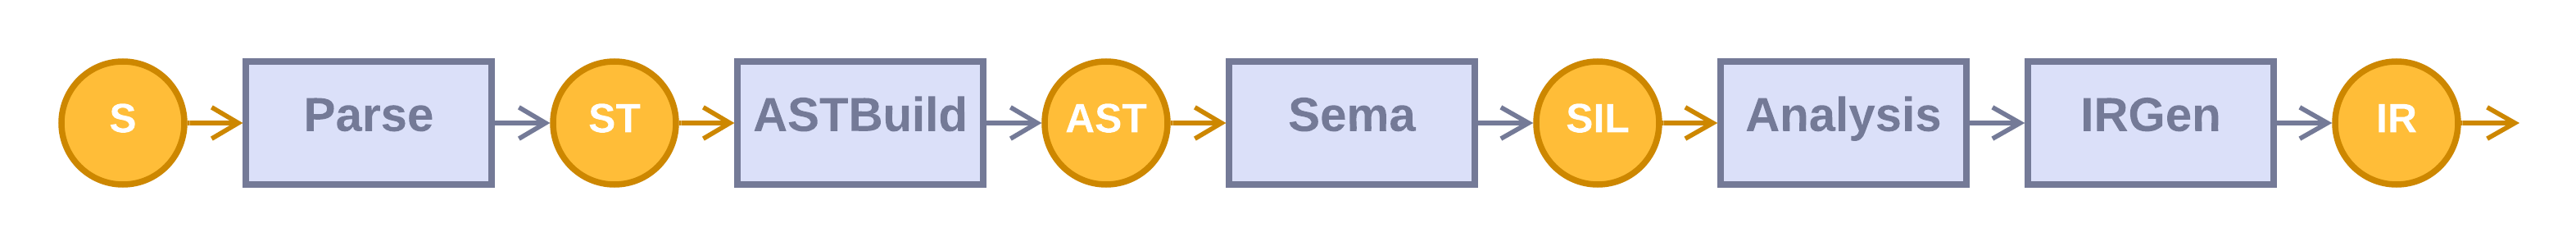
\includegraphics{shex-lite-process-01.png}
    \caption[High level view of the compiler flow]{High level view of the compiler flow.}
    \labfig{shex-lite-process-01}
\end{figure}

The \reffig{shex-lite-process-01} shows from a very high point of view a complete sequence of compilation
for the ShEx-Lite compiler. From there we can already capture that the compiler will be
composed of the following elements: 

\begin{itemize}
    \item \textbf{Parse:} Takes as input the source files and produces the Syntax Tree. 
    \item \textbf{ASTBuild:} Takes as an input the Syntax Tree and generates an Abstract Syntax Tree.
    \item \textbf{Sema:} From the Abstract Syntax Tree generated in the previous step it produces the ShEx-Lite Intermediate Language.
    \item \textbf{SIL Analysis:} Analyses the ShEx-Lite intermediate code and decides whether the corresponding Intermediate Representation can be dispatched or not.
    \item \textbf{IRGen:} Generates the corresponding Intermediate Representation.
\end{itemize}

Notice that those elements are independent one from another. Also from the \reffig{shex-lite-process-01}
we can already extract that the compiler will have at least the following structures:

\begin{itemize}
    \item \textbf{S:} Holds the Sources that the compiler will process. Those sources are \texttt{.shexl} files that contain the schemas that the user wants to compile.
    \item \textbf{ST:} Holds the output of the parse process. The parse process produces the Syntax Tree but also might generate warnings and errors. 
    \item \textbf{AST:} Contains the output of building the AST. This AST has not been type-checked nor annotated. 
    \item \textbf{SIL:} Contains the ShEx-Lite Intermediate Language. The SIL is the name for the typechecked annotated AST that has been transformed in to a graph structure. But it might also contains semantic error / warnings. 
    \item \textbf{IR:} Contains the generated Intermediate Representation. The IR is the sources that represent the generated domain object model, it contains those sources and all the compilation information. 
\end{itemize}

\begin{figure*}[hb]
    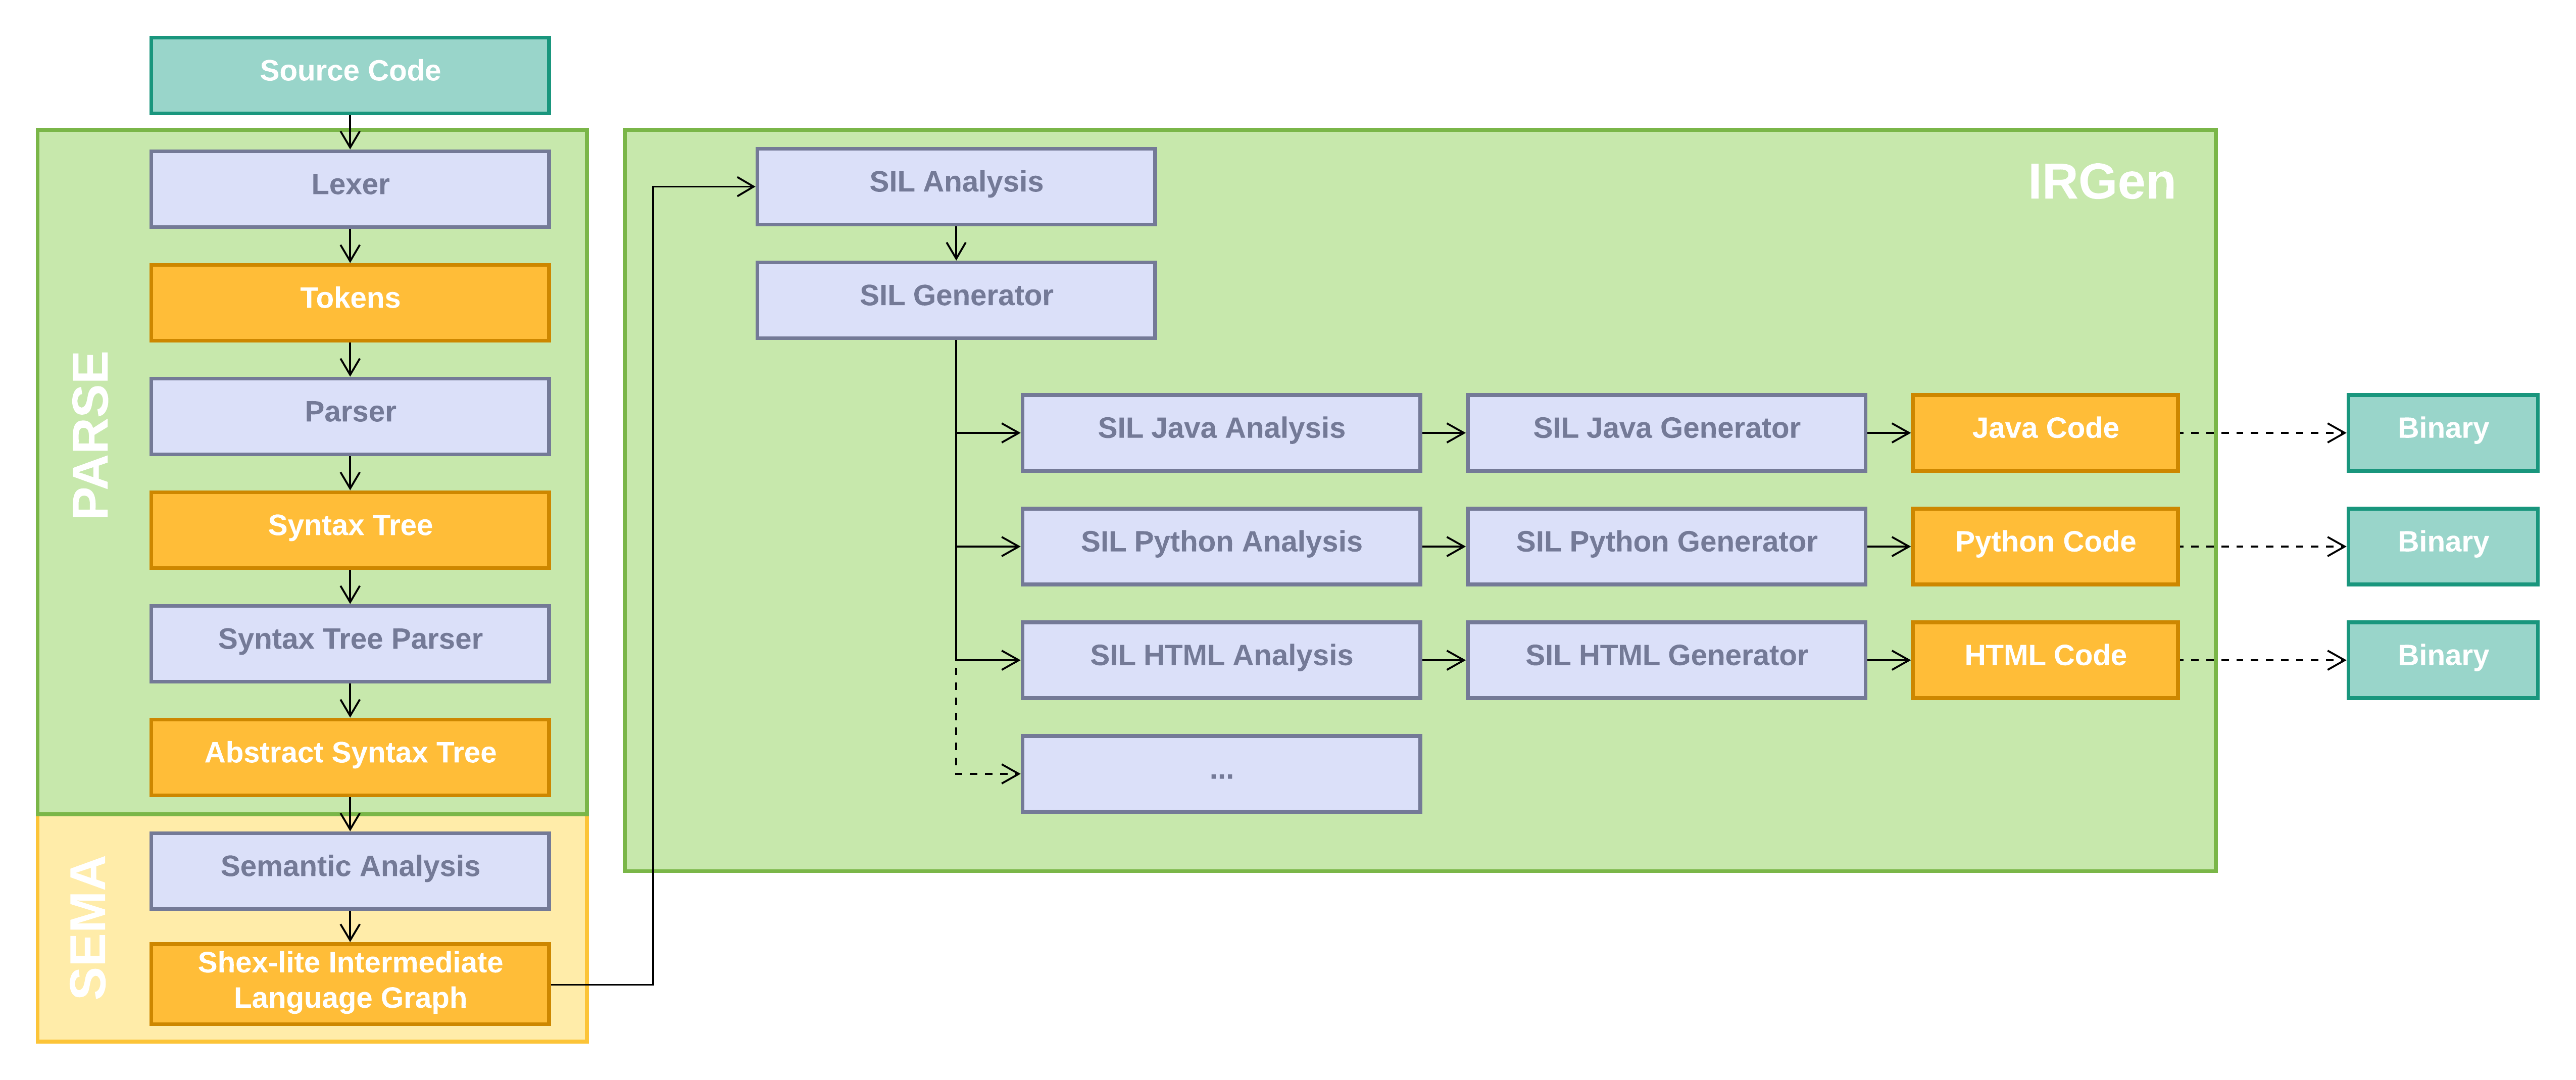
\includegraphics{shex-lite-process-02.png}
    \caption[Low level view of the compiler flow, grouped by compiler-action]{Low level view of the compiler flow, grouped by compiler-action.}
    \labfig{shex-lite-process-02}
\end{figure*}

From the \reffig{shex-lite-process-02} we can see that in the compiler each process (Parse, sema, …)
contains multiple components. For example the parse stage from \reffig{shex-lite-process-01} is composed
by a lexer and a parser, that will correspond with the first two components of the compiler
subsystem from \reffig{shex-lite-components}. This components will be deeply explored at the class diagram
section. 
\setchapterpreamble[u]{\margintoc}
\chapter{System Implementation}
\labch{system-implementation}

\section{ShEx-Lite Language Implementation}

\section{Compiler Implementation}
\setchapterpreamble[u]{\margintoc}
\chapter{Plannings and Budget}
\labch{plannings-budget}
\setchapterpreamble[u]{\margintoc}
\chapter{Conclusions}
\labch{conclusions}

\appendix % From here onwards, chapters are numbered with letters, as is the appendix convention

\pagelayout{wide} % No margins
\addpart{Annexes}
\pagelayout{margin} % Restore margins

\setchapterstyle{lines}
\labpage{shex-lite-lex-spec}
\chapter{ShEx-Lite Lexical Specification}
\setchapterstyle{lines}
\labpage{shex-lite-syntax-spec}
\chapter{ShEx-Lite Syntax Specification}

\begin{lstlisting}[basicstyle=\scriptsize]
    parser grammar ShexLiteParser;

    options { tokenVocab=ShexLiteLexer; }
    
    schema
     : statement+ EOF
     ;
    
    statement
     : import_stmt
     | definition_stmt
     ;
    
    import_stmt
     : IMPORT iri=literal_iri_value_expr
     ;
    
    definition_stmt
     : start_def_stmt
     | prefix_def_stmt
     | base_def_stmt
     | shape_def_stmt
     ;
    
    start_def_stmt
     : START EQ shape=call_shape_expr
     ;
    
    prefix_def_stmt
     : PREFIX IDENTIFIER? COLON iri=literal_iri_value_expr
     ;
    
    base_def_stmt
     : BASE iri=literal_iri_value_expr
     ;
    
    shape_def_stmt
     : label=call_prefix_expr expr=constraint_expr
     ;
    
    expression
     : literal_expr
     | cardinality_expr
     | constraint_expr
     ;
    
    literal_expr
     : literal_real_value_expr
     | literal_string_value_expr
     | literal_iri_value_expr
     ;
    
    literal_real_value_expr
     : DECIMAL_LITERAL
     ;
    
    literal_string_value_expr
     : STRING_LITERAL
     ;
    
    literal_iri_value_expr
     : IRI_LITERAL
     ;
    
    cardinality_expr
     : MUL
     | ADD
     | QUESTION
     | LBRACE min=DECIMAL_LITERAL RBRACE
     | LBRACE min=DECIMAL_LITERAL COMMA max=DECIMAL_LITERAL RBRACE
     | LBRACE min=DECIMAL_LITERAL COMMA RBRACE
     ;
    
    constraint_expr
     : constraint_node_expr
     | constraint_block_triple_expr
     | constraint_triple_expr
     ;
    
    constraint_node_expr
     : constraint_node_iri_expr
     | constraint_valid_value_set_type
     | constraint_node_any_type_expr
     | call_expr
     | constraint_node_non_literal_expr
     | constraint_value_set_expr
     | constraint_node_bnode_expr
     | constraint_node_literal_expr
     ;
    
    constraint_block_triple_expr
     : LBRACE (constraint_triple_expr)+ RBRACE
     ;
    
    constraint_triple_expr
     : property=call_prefix_expr constraint=constraint_node_expr cardinality=cardinality_expr? SEMI?
     ;
    
    constraint_node_iri_expr
     : IRI
     ;
    
    constraint_valid_value_set_type
     : call_prefix_expr
     | call_shape_expr
     | literal_string_value_expr
     | literal_real_value_expr
     ;
    
    constraint_node_any_type_expr
     : ANYTYPE
     ;
    
    constraint_node_non_literal_expr
     : NONLITERAL
     ;
    
    constraint_value_set_expr
     : LBRACK constraint_valid_value_set_type* RBRACK
     ;
    
    constraint_node_bnode_expr
     : BNODE
     ;
    
    constraint_node_literal_expr
     : LITERAL
     ;
    
    call_expr
     : call_prefix_expr
     | call_shape_expr
     ;
    
    call_prefix_expr
     : pref_lbl=IDENTIFIER? COLON shape_lbl=IDENTIFIER
     | base_relative_lbl=literal_iri_value_expr
     ;
    
    call_shape_expr
     : AT prefix_lbl=IDENTIFIER? COLON shape_lbl=IDENTIFIER
     | AT base_relative_lbl=literal_iri_value_expr
     ;
\end{lstlisting}
\setchapterstyle{lines}
\labpage{publications}
\chapter{Publications}

The research work of this End of Degree Project has been published in different conferences.
The following publications are shomehow derived from this E.D.F.

\begin{enumerate}
    \item \textbf{ASIO: a Research Management System based on Semantic technologies.} Jose Emilio Labra Gayo,
    José Barranquero Tolosa, Guillermo Facundo Colunga, Alejandro González Hevia, Emilio Rubiera Azcona and
    Paulino Álvarez de Ron Ondina.
    \item \textbf{ShEx-Lite: Automatic generation of domainobject models from Shape Expressions.} Guillermo Facundo Colunga,
    Alejandro González Hevia, Jose Emilio Labra Gayo and Emilio Rubiera Azcona.
    \item \textbf{Automatic synchronization of RDF graphs and a Wikibase instance.} Alejandro González Hevia,
    Guillermo Facundo Colunga, Emilio Rubiera Azcona and Jose Emilio Labra Gayo.
    \item \textbf{El que nos falta a alejandro y a mi general.} Guillermo Facundo Colunga,
    Alejandro González Hevia, Jose Emilio Labra Gayo and Emilio Rubiera Azcona.
\end{enumerate}

%----------------------------------------------------------------------------------------

\backmatter % Denotes the end of the main document content
\setchapterstyle{plain} % Output plain chapters from this point onwards

%----------------------------------------------------------------------------------------
%	BIBLIOGRAPHY
%----------------------------------------------------------------------------------------

% The bibliography needs to be compiled with biber using your LaTeX editor, or on the command line with 'biber main' from the template directory

\defbibnote{bibnote}{Here are the references in citation order.\par\bigskip} % Prepend this text to the bibliography
\printbibliography[heading=bibintoc, title=References, prenote=bibnote] % Add the bibliography heading to the ToC, set the title of the bibliography and output the bibliography note

%----------------------------------------------------------------------------------------
%	NOMENCLATURE
%----------------------------------------------------------------------------------------

% The nomenclature needs to be compiled on the command line with 'makeindex main.nlo -s nomencl.ist -o main.nls' from the template directory

\nomenclature{$c$}{Speed of light in a vacuum inertial frame}
\nomenclature{$h$}{Planck constant}

\renewcommand{\nomname}{Notation} % Rename the default 'Nomenclature'
\renewcommand{\nompreamble}{The next list describes several symbols that will be later used within the body of the document.} % Prepend this text to the nomenclature

\printnomenclature % Output the nomenclature

%----------------------------------------------------------------------------------------
%	GREEK ALPHABET
% 	Originally from https://gitlab.com/jim.hefferon/linear-algebra
%----------------------------------------------------------------------------------------

\vspace{1cm}

{\usekomafont{chapter}Greek Letters with Pronounciation} \\[2ex]
\begin{center}
	\newcommand{\pronounced}[1]{\hspace*{.2em}\small\textit{#1}}
	\begin{tabular}{l l @{\hspace*{3em}} l l}
		\toprule
		Character & Name & Character & Name \\
		\midrule
		$\alpha$ & alpha \pronounced{AL-fuh} & $\nu$ & nu \pronounced{NEW} \\
		$\beta$ & beta \pronounced{BAY-tuh} & $\xi$, $\Xi$ & xi \pronounced{KSIGH} \\
		$\gamma$, $\Gamma$ & gamma \pronounced{GAM-muh} & o & omicron \pronounced{OM-uh-CRON} \\
		$\delta$, $\Delta$ & delta \pronounced{DEL-tuh} & $\pi$, $\Pi$ & pi \pronounced{PIE} \\
		$\epsilon$ & epsilon \pronounced{EP-suh-lon} & $\rho$ & rho \pronounced{ROW} \\
		$\zeta$ & zeta \pronounced{ZAY-tuh} & $\sigma$, $\Sigma$ & sigma \pronounced{SIG-muh} \\
		$\eta$ & eta \pronounced{AY-tuh} & $\tau$ & tau \pronounced{TOW (as in cow)} \\
		$\theta$, $\Theta$ & theta \pronounced{THAY-tuh} & $\upsilon$, $\Upsilon$ & upsilon \pronounced{OOP-suh-LON} \\
		$\iota$ & iota \pronounced{eye-OH-tuh} & $\phi$, $\Phi$ & phi \pronounced{FEE, or FI (as in hi)} \\
		$\kappa$ & kappa \pronounced{KAP-uh} & $\chi$ & chi \pronounced{KI (as in hi)} \\
		$\lambda$, $\Lambda$ & lambda \pronounced{LAM-duh} & $\psi$, $\Psi$ & psi \pronounced{SIGH, or PSIGH} \\
		$\mu$ & mu \pronounced{MEW} & $\omega$, $\Omega$ & omega \pronounced{oh-MAY-guh} \\
		\bottomrule
	\end{tabular} \\[1.5ex]
	Capitals shown are the ones that differ from Roman capitals.
\end{center}

%----------------------------------------------------------------------------------------
%	GLOSSARY
%----------------------------------------------------------------------------------------

% The glossary needs to be compiled on the command line with 'makeglossaries main' from the template directory

\newglossaryentry{computer}{
	name=computer,
	description={is a programmable machine that receives input, stores and manipulates data, and provides output in a useful format}
}

% Glossary entries (used in text with e.g. \acrfull{fpsLabel} or \acrshort{fpsLabel})
\newacronym[longplural={Frames per Second}]{fpsLabel}{FPS}{Frame per Second}
\newacronym[longplural={Tables of Contents}]{tocLabel}{TOC}{Table of Contents}

\setglossarystyle{listgroup} % Set the style of the glossary (see https://en.wikibooks.org/wiki/LaTeX/Glossary for a reference)
\printglossary[title=Special Terms, toctitle=List of Terms] % Output the glossary, 'title' is the chapter heading for the glossary, toctitle is the table of contents heading

%----------------------------------------------------------------------------------------
%	INDEX
%----------------------------------------------------------------------------------------

% The index needs to be compiled on the command line with 'makeindex main' from the template directory

\printindex % Output the index

%----------------------------------------------------------------------------------------
%	BACK COVER
%----------------------------------------------------------------------------------------

% If you have a PDF/image file that you want to use as a back cover, uncomment the following lines

%\clearpage
%\thispagestyle{empty}
%\null%
%\clearpage
%\includepdf{cover-back.pdf}

%----------------------------------------------------------------------------------------

\end{document}
